\documentclass[]{article}

\usepackage{amsmath}
\usepackage{siunitx}
\usepackage{diffcoeff}
\usepackage{graphicx}
\usepackage[space]{grffile}
\usepackage{url}
\usepackage{enumitem}
\usepackage{pythontex}
\usepackage{appendix}
\usepackage{etoolbox}
\usepackage{pmboxdraw}
%\usepackage[utf8]{inputenc}
\usepackage{pythonhighlight}
\usepackage{relsize}
\usepackage[hidelinks]{hyperref}
\usepackage[all]{hypcap}
\usepackage{prettyref,cleveref}
\usepackage[margin=1.0in]{geometry}
\usepackage{mathtools}
\usepackage{cancel}
\usepackage{parskip}
\usepackage{placeins}
\usepackage{subfig}
\usepackage{bigints}
\usepackage[style=numeric, backend=biber]{biblatex}
\usepackage{fontspec}
\usepackage[mathbf=sym, warnings-off={mathtools-colon,mathtools-overbracket}]{unicode-math}
\usepackage{bm}
\usepackage{comment}
\usepackage{xspace}
\usepackage{xpatch}
\usepackage{array,makecell}
\usepackage{rotating}

\usepackage[nolist,nohyperlinks]{acronym}
\usepackage{glossaries}
\makeglossaries

\usepackage{nomencl}
\makenomenclature

\usepackage{todonotes}

%\addbibresource{'Plasma-Transport-Code.bib'}
\addbibresource{Plasma-Transport-Code.bib}

% Nomenclature adjustments
\usepackage{etoolbox, ragged2e}
\renewcommand\nomgroup[1]{%
	\item[\bfseries
	\ifstrequal{#1}{P}{Parameters}{%
		\ifstrequal{#1}{S}{Subscripts}{%
			\ifstrequal{#1}{C}{Constants}{}}}%
	]}

\setlength\nomlabelwidth{2cm}

\patchcmd{\thenomenclature}
{\leftmargin\labelwidth}
{\leftmargin\labelwidth\itemindent 2em }
{}{}

\newcommand{\DimensUnits}[2]{%
	\quad
	\parbox[t]{16em}{\RaggedRight #1}%
	\quad
	\makebox[4em][l]{#2}%
}

\newcommand{\insertnomheaders}{%
	\item[\bfseries Symbol]
	\nomdescr{\textbf{Quantity}}\DimensUnits{\textbf{Dimension}}{\textbf{Unit}}%
}
\renewcommand{\nomname}{Nomenclature and Dimensions}

\renewcommand\nomgroup[1]{\item[\large\bfseries]\insertnomheaders}

\newcommand{\nomdescr}[1]{\parbox[t]{6cm}{\RaggedRight #1}}
\newcommand{\symdef}[4]{\nomenclature{#1}{\nomdescr{#2}\DimensUnits{#3}{#4}}}

% Nomenclature adjustments

% This will add the units
%----------------------------------------------
\newcommand{\nomunit}[1]{%
	\renewcommand{\nomentryend}{\hspace*{\fill}#1}}
%----------------------------------------------
% \setmathfont{Cambria}

%\newcommand{\emath}[1]{\ensuremath{#1}}

\renewcommand{\CancelColor}{\color{blue}} %change cancel color to red

\setlength{\parskip}{1em}


\setcounter{section}{0} 

\setcounter{secnumdepth}{4}

\crefname{section}{Section}{Sections}
\crefname{subsection}{Section}{Sections}
\crefname{susubsection}{Section}{Sections}
\crefname{paragraph}{Section}{Sections}
\crefname{equation}{Equation}{Equations}
\crefname{figure}{Figure}{Figures}
\crefname{table}{Table}{Tables}
\crefname{listing}{Listing}{Listings}
\newrefformat{eq}{Equation \ref{#1} on page \pageref{#1}}


\def \figpath {"Images/"}

\def \diffpfunc #1#2{\diffp*{\left(\vphantom{\diffp*{}#2}#1\right)}#2}
%\diffp*{\left( \vphantom{\diffp*{}#2}#2 #1 \right)}#1 \right)
\def \func #1#2{#1\left(\vphantom{#1} #2\right)}
\def \FrIOL #1{\func{ F_{#1\vphantom{j}}^\mathrm{iol} }{r}} % Using Phantom J to ensure parens for both j and k are same size
\def \flux #1{\func{ \Gamma_{r#1}}{r} }

% Inserts \clearpage before \begin{appendices}
%\BeforeBeginEnvironment{appendices}{\clearpage}
% Inserts \clearpage after \end{appendices}
%\AfterEndEnvironment{appendices}{\clearpage}

% Inserts \clearpage before every \section within appendices environment
\AtBeginEnvironment{appendices}{\pretocmd{\section}{\clearpage}{}{}}{}
\newcommand\mytodo[1]{\textcolor{red}{#1}}


\newcommand{\csubfloat}[2][]{%
	\makebox[0pt]{\subfloat[#1]{#2}}%
}
\newcommand{\centerhfill}[1][\quad]{\hspace{\stretch{0.5}}#1\hspace{\stretch{0.5}}}

\newcommand*{\vxb}{\ensuremath{\vec{V} \times \vec{B}}\xspace}





%opening
\title{A Transport Solution for Plasma Fluid Equations that Conserves Particles, Momentum, \& Energy}
\author{E. William DeShazer}                                                                                                                                                                                                                                                                                                                                                                                                                                                                                                                                                                                                                                                                                                                                                                                                                                                                                                                                                                                                                                                
\date{\today}

%\todo{Fix}:Reduce right margin for nomenclature
%\nomenclature[P]{$r$}{Radial location along the minor radius}
%\nomenclature[P]{$\hat{\Gamma}$}{Radial flux \nomunit{$\cfrac{1}{s\cdot sr}$}}
%\nomenclature[P]{$S_n$}{Particle source}
%\nomenclature[P]{$F^{IOL}$}{Thermal Ion Orbit Loss fraction}
%\nomenclature[P]{$\alpha, \beta$}{Charge neutrality adjustment term}
%\nomenclature[P]{$f^{IOL}$}{Fast Ion Orbit Loss fraction}
%\nomenclature[P]{$z$}{Atomic Number}
%\nomenclature[P]{$N_{nb}$}{Fast Neutral Beam Source Rate}
%\nomenclature[P]{$\hat{\alpha}$}{description}
%\nomenclature[P]{$\nu_{ion}$}{Frequency of Ionization}
%\nomenclature[P]{$n$}{Species number density}
%\nomenclature[P]{$L_p^{-1}$}{Pressure Gradient Scale Length $\frac{1}{p} \diffp{p}{r}$ }
%\nomenclature[P]{$L_T^{-1}$}{Temperature Gradient Scale Length $\frac{1}{T} \diffp{T}{r}$ }
%
%\nomenclature[S]{nbi}{Neutral Beam Injection}
%\nomenclature[S]{$j$}{Primary Ion}
%\nomenclature[S]{$k$}{Impurity Ion}
%\nomenclature[S]{$r$}{Radial Component}
%\nomenclature[S]{$e$}{Electron}

%\symdef{$\pi$}{length}{\frac{M}{s}}{\si{m}}
%\symdef{$\alpha$}{angle}{L}{\si{F.m^{-1}}}
%\symdef{$\beta$}{another length}{meter}{\si{v}}
\newglossaryentry{L-Mode}
{ 	name=L-Mode, 
	description={Short for Low Mode, an operational regime characterized by a shallow pressure, density, and temperature pedestal}
}

\newglossaryentry{H-Mode}
{	name=H-Mode,
	description={Short for High Mode, an operational regime characterized by a steep pressure, density, and temperature pedestal}
}

\newglossaryentry{SH-Mode}
{	name=SH-Mode,
	description={Short for Super High Modee, an operational regime with an elevated pedestal pressure relative to H-Mode}
}

\newglossaryentry{NT-Mode}
{	name=NT-Mode,
	description={Short for Negative Triangularity Mode, an operational regime characterized by a D-shaped cross-section that points radially inward (major axis) rather than the more common radially outward facing D-shape}
}

\newglossaryentry{SOL}{
	name={SOL},
	description={A region outside of the \ac{LCFS} that serves as the exhaust for tokamak plasmas. It derives its name from the early tokamak designs that put a physical barrier known as a limiter in the region to "scrape" off the outer layer of the plasma. The limiter design has mostly been replaced with the divertor design but this plasma region retains the same designation.}
}

\begin{acronym}
	\acro{RMP}{Reverse Magnetic Pinch}
	\acro{IOL}{Ion Orbit Loss}
	\acro{NBI}{Neutral Beam Injection}
	\acro{CX}{Charge Exchange}
	\acro{SOL}{Scrape-off Layer}
	\acro{LCFS}{Last Closed Flux Surface}
	\acro{GIT}{Georgia Institute of Technology}
	\acro{FRC}{Fusion Research Center}
	\acro{ODE}{Ordinary Differential Equation}
	\acro{FSA}{Flux Surface Average}
	\acro{SOL}{Scrape-off Layer}
	\acro{GMRES}{Generalized Minimal Residual Method}
	\acro{TEP}{Transport Escape Probability}
	\acro{ITB}{Interface Current Balance}
\end{acronym}

\begin{document}

\maketitle

\mbox{}

\begin{abstract}
	A predictive transport computational model that solves a recently postulated form of the plasma fluid equations \cite{Stacey2017} that conserves particles, momentum, and energy will be implemented. The transport equations set will be extended and modified as necessary to provide reasonable agreement with experimental data collected from DIII-D, a research tokamak owned by General Atomics. Thus, a validation exercise comparing against a variety of H-mode, L-Mode and RMP data sets is anticipated in the development of the computational model. The transport equations were proposed to capture the radial distribution resulting from a neutral beam source, which inserts particles, momentum, and energy, ion orbit loss, which removes particles and their associated momentum and energy in a non-diffusive manner, and the equilibrium field conditions of toroidal and poloidal rotation velocities, plasma pressure, density, and temperature. The equations as presented are first order, coupled, non-linear equations, resulting from the long range Lorentz forces $\left(\vxb\right)$ and electric field $\left(\vec{E}\right)$. Therefore, iterative computational techniques will be employed. The primary solver that will be explored is a variant of the Newton-Raphson multivariate solver known as Broyden’s method. A pure Newton-Raphson solver evaluates the Jacobian analytically, but the nature of our equations will require a numerical approximation of the Jacobian. In the course of the analysis if other iterative techniques arise, we will consider implementing them for comparison.
\end{abstract}


\section{Introduction} \label{sec:Introduction}

The path toward fusion as an energy source hinges on an understanding and description of the plasma dynamics. On the experimental side, great effort is being given to access and exploit high performance operational regimes such as \gls{H-Mode}\cite{Loarte2011}, \gls{SH-Mode}\cite{Knolker2020} (\prettyref{fig:superhmode}) and the most recent addition, \gls{NT-Mode}\cite{Marinoni2020, Medvedev2015} (\prettyref{fig:standared-d-vs-negative-d}). Each of these regimes show improved plasma performance characteristics in the form of longer confinement times, but many codes, including SOLPS, UEDGE, or ONETWO, satisfy fluid conservation equations in the absence of electromagnetic effects. Instead these codes assume diffusion as the primary transport mechanism and impose electromagnetic effects after the equilibrium field has been solved. One of the key weaknesses in this modeling approach is diffusion implies that particles move down the pressure gradient, whereas the aforementioned regimes should exhibit increased transport in the presence of steep pressure gradients at the plasma edge. In fact, they exhibit exactly the opposite.

\begin{figure}[!ht]
	\subfloat[Pedestal Bifurcation during Super H-Mode in Density Space \cite{Knolker2020}] {
		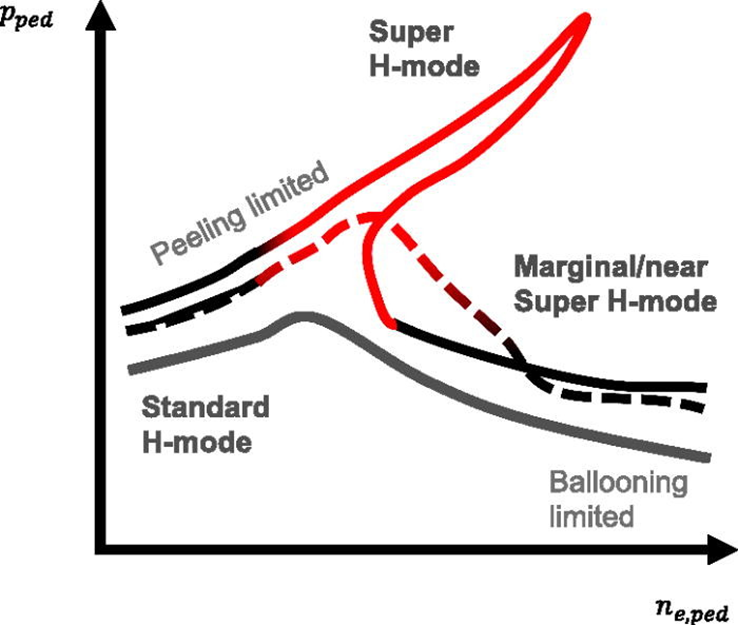
\includegraphics[width=0.45\linewidth]{images/PedBifurcationSuperHmode}
		\label{fig:superhmode}
	} \quad
	\subfloat[Equilibrium configurations and \ac{SOL} flow patterns for (a) standard D-shaped tokamak and (b) negative triangularity snowflake divertor tokamak \cite{Medvedev2015}] {
		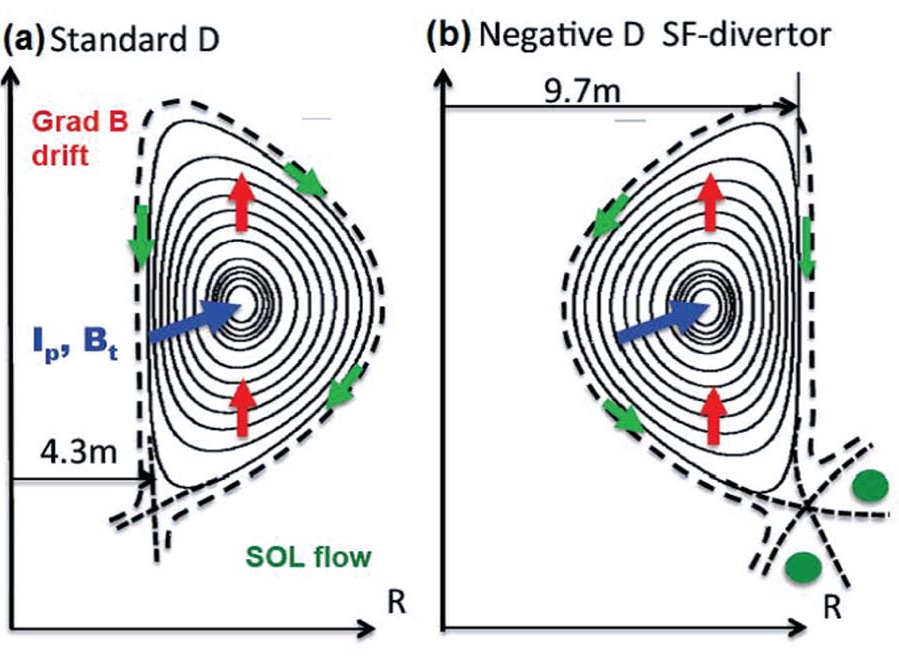
\includegraphics[width=0.5\linewidth]{images/Standard_D_vs_Negative_D}
		\label{fig:standared-d-vs-negative-d}
	}
	\caption{High Performance Operational Regimes}
\end{figure}

Within the plasma community it is known that the exhibited improved performance implies a pinch effect, but a satisfying descriptive model to explain these effects has been elusive. The fluid equations as proposed by \citeauthor{Stacey2017} \cite{Stacey2017} and outlined in \cref{sec:Theory} has the pleasing feature that the long-range \vxb forces are retained in the momentum conservation equations \cref{sub:MomentumConservation} while introducing a more theoretically sound mechanism for particle loss in the form of \ac{IOL}, both thermal and fast. 

The justification that \ac{IOL} is more theoretically sound arises from the observation that diffusion, a near-field effect that is driven by pressure gradients, is an inherently collisional transport mechanism. However, central to the theory of a plasma is that it is most assuredly not. The \ac{IOL} argument is that the particles within a flux surface, to a first order, satisfy conservation canonical angular momentum, energy, and magnetic moment, as will be discussed in \cref{sub:IOL}. The flux surface energy, in the form of temperature, is a Maxwellian distribution, which means particles in the tail, have sufficient energy to take particles beyond the \ac{LCFS}. Both magnetic field irregularities and physical barriers, such as walls, result in particles being removed while trying to execute orbits. 

The inclusion of long-range \vxb forces into the momentum conservation as discussed in \cref{sub:MomentumConservation} is satisfying because it forces the equilibrium solution for the pressure field to re-balance in the presence of the fluid velocities, both the toroidal, $V_\psi$, and poloidal, $V_\theta$.

The fluid theory presented in this paper has developed in some form at the \ac{GIT} \ac{FRC} for as long as fusion has been actively researched there. However, the effort to fully describe the physics in the edge and pedestal region were outlined in \citetitle{Stacey2003}\cite{Stacey2003}.  Stacey and Groebner lay out the physics constraints that are important to an plasma edge/pedestal model in Section II and detail a road-map on the work required realize the ultimate goal stated in Section VI, a fully predictive pedestal model. 

The formal statement of this fluid theory appears first in \citetitle{Stacey2004} from \citeauthor{Stacey2004}\cite{Stacey2004}. Many of the modeling assumptions, such as the observation that a phase space integration of the generalized continuity equation results in only a radially flux or the form of the effective diffusion coefficient, are presented. In a series of several papers, \cite{Stacey2008, Stacey2012, Floyd2012, Wilks2016}, the transport formalism that is being studied in this paper was used to interpret particle flux, \ac{IOL}, and intrinsic rotation based on experimental input of density and temperature. In fact, the model was shown to have an agreement with experimental rotation velocity data from DIII-D to within 10-20\%\cite{Stacey2012}.

The next step, and the objective of this research, is the final step of the 2003 paper \cite{Stacey2003}  is to produce a predictive transport model that conserves particles, momentum and energy by including the non-diffusive loss mechanism of \ac{IOL} and retaining the long range electromagnetic contributions of \vxb. A necessary and intermediate step is to provide an iterative computational algorithm that is compatible with the strong E\&M and \vxb forces simultaneously with the weaker scattering forces. To this end, we will explore the Broyden algorithm, a quasi Newton-Raphson method, as the primary iterative solver in combination with Gauss reduction. A validation exercise against a variety of operational modes, \gls{L-Mode}, \gls{H-Mode}, \gls{NT-Mode}, and \ac{RMP} is envisioned. The result will be a code that predicts the radial density, pressure, and temperature fields as well as the associated toroidal and poloidal velocities.


\subsection{Regions of a Tokamak Plasma} \label{sub:RegionsOfPlasma}

\begin{figure}
	\centering
	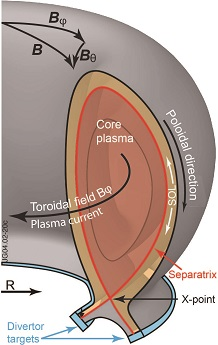
\includegraphics[width=0.5\linewidth]{images/RegionsOfaTokamakPlasma}
	\caption[Features of a Tokamak Plasma\cite{LipschultzBandSharples}]{}
	\label{fig:featuressofatokamakplasma}
\end{figure}

High level features of a tokamak plasma are illustrated in the \prettyref{fig:featuressofatokamakplasma}. These regions include the Core Plasma, the \acf{SOL}, which will sometimes be referred to as the edge region, the Separatrix, which will also be referred to as the \acf{LCFS}, and the X-Point, which is a feature of a divertor design. Also illustrated in this figure is the major radius, R, which is measured from the central axis of the torus. The toroidal direction, $\varphi$, and the poloidal direction are represented. In accordance with these directions, the magnetic field $\vec{B}$ is decomposed into a direction aligned with the toroidal direction, $\vec{B_\varphi}$ and a component that is in the poloidal direction, $\vec{B_\theta}$. Velocity can be decomposed as either parallel to $\vec{B}$, $\left(V_\parallel\right)$, perpendicular to $\vec{B}$, $\left(V_\perp\right)$ or along one of the toroidal directions $\left(V_\varphi \text{ or } V_\varTheta\right)$. The minor axis, r, which is not illustrated here, extends from the plasma magnetic center to the outer wall. For this reason, the radius that works its way into equations is not a fixed value but is given by \cref{eqn:Radius}
%
\begin{equation}
	R\left(r\right) = R_0 + r\cos \theta
	\label{eqn:Radius}
\end{equation}
%
where, $R_0$ is the radial distance from toroidal center to the magnetic center. Because, this analytical approach is one-dimensional $\theta = 0$ and $R\left(r\right)$ is simply $R_0 + r$


\section{Theory} \label{sec:Theory}

The fundamental parts of the predictive model are the conservation of particles (\cref{sub:ParticleConservation}), momentum (\cref{sub:MomentumConservation}), and energy (\cref{sub:EnergyConservation}), the conduction closure (\cref{sub:ConductionClosure}) and the ideal gas law (\cref{sub:IdealGasLaw}). Within each of the conservation equations there is provision for the removal of particles, momentum, and energy due to \ac{IOL}, which is described in \cref{sub:IOL}. \ac{IOL} calculation requires input from the equilibrium reconstruction. Therefore, a short overview is provided in \cref{subsub:EFIT}.  The primary source of particles, momentum, and energy considered is beam input and therefore, details on the beam modeling are covered in \cref{sub:BeamModeling}. Finally, the pinch diffusion model is described, because there is a desire to recast the conservation equations in the form of a pinch diffusion equation. Therefore, the pinch diffusion model will be discussed in \cref{sub:PinchDiffusion}

\subsection{Conservation of Particles} \label{sub:ParticleConservation}

The general multidimensional form of the continuity equation in \cref{eqn:GeneralContinuity}
%
\begin{equation}
	\symbf{\nabla} \cdot n_j \symbf{v}_j = S_j
	\label{eqn:GeneralContinuity}
\end{equation}
%
reduces to the one-dimensional non-linear \ac{ODE} shown in \cref{eqn:Continuity} and \cref{eqn:Source} when one performs a \ac{FSA}. The reason is that the poloidal component of the flux, $\langle \left(\symbf{\nabla} \cdot n_j \symbf{v}_j \right)_\theta \rangle = 0$ identically and $\langle \left(\symbf{\nabla} \cdot n_j \symbf{v}_j \right)_\phi \rangle = 0$ by axisymmetry \cite{Stacey2004}.

\begin{equation}
	\cfrac{1}{r} \diffpfunc{ r \func{\Gamma_{rj}}{r}}{r} =
	S_{nj} -\alpha \diffpfunc{ \FrIOL{j} }{r} \flux{j}
	-\beta z_{k} \diffpfunc{ \FrIOL{k} }{r} \flux{k}
	\label{eqn:Continuity}
\end{equation}
%
where,
%
\begin{equation}
	S_{nj} \equiv \func{N_\mathrm{nbj}}{r} \left( 1\ -\hat{\alpha } \func{f^\mathrm{iol}_\mathrm{nbi}}{r} \right)+ \func{n_{e}}{r} \nu _{\mathrm{ion}_j} (r)
	\label{eqn:Source}
\end{equation}

The left side of \cref{eqn:Continuity} expresses the change in flux, $\Gamma_{rj}$ of the primary ion is driven by the source terms on the right. First, $S_{nj}$, is the positive contributions due to \ac{NBI} and ionization. In \cref{eqn:Source}, $N_{nbj}$ is the rate of \ac{NBI} injection, which has been reduced by the fast \ac{IOL}, $f^\mathrm{iol}_\mathrm{nbi}$. The rate of neutral beam injection is based on a beam model that is described in \cref{sub:BeamModeling}. The second term, $\func{n_{e}}{r} \nu _{\mathrm{ion}_j} (r)$ is the ionization rate and is discussed in \cref{sub:NeutralTransport}. Lastly, in \cref{eqn:Continuity}, there are two terms for \ac{IOL}, $\FrIOL{j}$ for the primary ion, and $\FrIOL{k}$ for the impurity ion. They are the cumulative loss of ions through the mechanism of \ac{IOL}. They impact the conservation of particles through their differential contributions, $\diffp{}{r}$. These \ac{IOL} terms are detailed in \cref{sub:IOL}. The terms, $\alpha$ and $\beta$ are charge neutrality adjustment terms and will be a subject of consideration. There are three mechanisms by which the charge associated with lost primary ions can be compensated:

\begin{enumerate}[label=(\roman*)]
	\item A commensurate lost electrons implying $\left(\alpha=1, \beta=0\right)$ thus nullifying $\FrIOL{k}$, \label{item:NeutElectron}
	\item A return current of thermalized ions from the \ac{SOL} (\gls{SOL}) implying $\left(\alpha=2, \beta=1\right)$, or \label{item:NeutImpurity}
	\item No \ac{IOL} $\left(\alpha=0, \beta=0\right)$ \label{item:NeutNoIOL}
\end{enumerate}

\citeauthor{Stacey2017} conjectures that the most physically reasonable is \cref{item:NeutImpurity}, which we intend to explore.


%\symdef{$r$}{Location along the minor radius}{\emath{L}}{$m$}
%\nomenclature{$\hat{\Gamma}_{rj}$}{Radial flux for primary ion j}{L}{dum}
%\nomenclature{$S_n$}{Particle source}
%\nomenclature{$F^{IOL}$}{Thermal Ion Orbit Loss fraction}
%\nomenclature{$\alpha, \beta$}{Charge neutrality adjustment term}
%\nomenclature{$f^{IOL}$}{Fast Ion Orbit Loss fraction}
%\nomenclature{$z$}{Atomic Number}
%\nomenclature{$N_{nb}$}{Fast Neutral Beam Source Rate}
%\nomenclature{$\hat{\alpha}$}{description}
%\nomenclature{$\nu_{ion}$}{Frequency of Ionization}
%\nomenclature{$n$}{Species number density}
%\nomenclature{$L_p^{-1}$}{Pressure Gradient Scale Length $\frac{1}{p} \diffp{p}{r}$ }
%\nomenclature{$L_T^{-1}$}{Temperature Gradient Scale Length $\frac{1}{T} \diffp{T}{r}$ }

%\subsection{Ion Orbit Loss} \label{sub:IOL}

\acf{IOL} represents a non-diffusive mechanism for losing particles. At the heart of \ac{IOL} theory is an electromagnetic equilibrium argument that, to a first order, between any two flux surfaces canonical angular momentum (\cref{eqn:IOLCanonAngleMom}), energy (\cref{eqn:IOLEnergy}), and magnetic moment (\cref{eqn:IOLMagMom}) are conserved. Based on this fundamental principle, \citeauthor{Miyamoto1996} \cite{Miyamoto1996} observed that one could use the values of plasma parameters on an inner flux surface (marked with a subscript 0) and the parameters on a separatrix, (marked with a subscript s or no subscript). \prettyref{fig:featuressofatokamakplasma} illustrates two flux surfaces, one being the separatrix and an inner one between the core and edge region.

\begin{equation}
	\left[ R\, m\, V_\parallel \left(\cfrac{B_\varphi}{B}\right) + e \psi \right]_0
	=
	\left[ R\, m\, V_\parallel \left(\cfrac{B_\varphi}{B}\right) + e \psi \right]_s 
	\label{eqn:IOLCanonAngleMom}
\end{equation}

\begin{equation}
	\left[ \cfrac{1}{2} \left( V_\parallel^2 + V_\perp^2  \phantom{\cfrac{1}{2}}\right) \right]_0
	=
	\left[ \cfrac{1}{2} \left( V_\parallel^2 + V_\perp^2  \phantom{\cfrac{1}{2}}\right) \right]_s
	\label{eqn:IOLEnergy}	
\end{equation}

\begin{equation}
	\left[ \cfrac{m\,V_\perp^2}{2\,B} \right]_0
	=
	\left[ \cfrac{m\,V_\perp^2}{2\,B} \right]_s
	\label{eqn:IOLMagMom}
\end{equation}

Utilizing \cref{eqn:IOLV0}, defining the term $f_\varphi$ in \cref{eqn:IOLfphi} and the parameter $\zeta_0$, which is the direction cosine of the particles launch angle with respect to the toroidal magnetic field line, $B_\varphi$, \crefrange{eqn:IOLCanonAngleMom}{eqn:IOLMagMom} can be rewritten into \cref{eqn:IOLMinV0}. This equation, which is quadratic in $V_0$, represents the equilibrium velocity for a particle to have an orbit that is within the confined portion of the plasma, meaning within the separatrix.

\begin{equation}
	V_0 = \sqrt{V_\parallel^2 + V_\perp^2}
	\label{eqn:IOLV0}
\end{equation}

\begin{equation}
	f_\varphi = \left|\cfrac{B_\varphi}{B}\right|
	\label{eqn:IOLfphi}
\end{equation}

\begin{equation}
	\zeta_0 = \cfrac{V_{\parallel 0}}{V_0}
	\label{eqn:IOLzeta0}
\end{equation}

This then serves as the criterion for which a particle can be lost. If it has an energy in excess of this, then it will have an orbit outside of the confined plasma and can encounter a variety of obstructions, such as magnetic field imperfections, \ac{SOL} particles, and most obviously, the wall. The manner by which this minimum velocity is applied to calculate a loss estimate is described in \cref{subsub:CumulativeLoss}.

\begin{equation}
	\begin{gathered}
			V^2_0 \left[ \left( \cfrac{R_0}{R} \cfrac{f_{\varphi 0}}{f_{\varphi}} \zeta_0 \right)^2 -1 + 
		\left( 1 - \zeta^2_0 \right) \left| \cfrac{B}{B_0} \right|  \right] + 
		V_0 \left[ \cfrac{2e \left( \psi_0 - \psi \right) }{R m f_\varphi} \left( \cfrac{R_0}{R}  \cfrac{f_{\varphi 0}}{f_\varphi} \zeta_0 \right)^{\vphantom{2}}   \right] \\
		+ \left[ \left( \cfrac{e\left( \psi_0 - \psi \right) }{R m f_\varphi} \right)^2 - \cfrac{2 e \left(\phi_0 - \phi  \right) }{m} \right] = 0
	\end{gathered}
	\label{eqn:IOLMinV0}
\end{equation}

\prettyref{fig:iolCalc} shows the minimum energy calculations against plasma ion temperature, what this illustrates is that \ac{IOL} is not a dominant transport mechanism for the plasma core. However, it becomes the dominant effect in the last 5\% \cite{Stacey2013} and drives the features in this region.

\begin{figure}
	\centering
	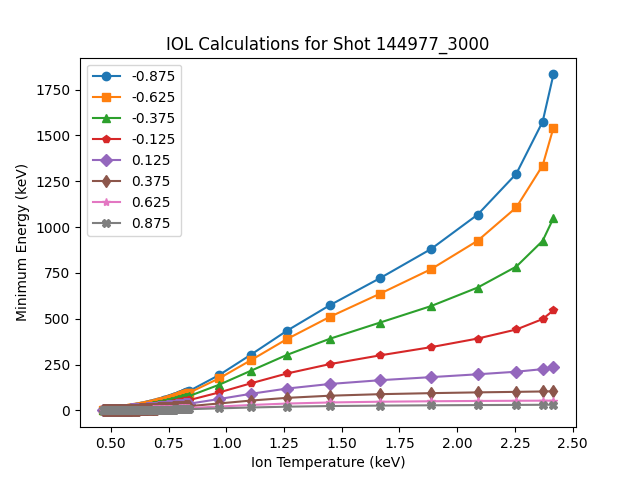
\includegraphics[width=0.5\linewidth]{images/iol_calculations}
	\caption[IOL Calculation]{Minimum Energy calculation for Shot 144977.3000}
	\label{fig:iolCalc}
\end{figure}


\subsubsection{Cumulative Loss Fraction} \label{subsub:CumulativeLoss}

The temperature of any flux surface is assumed to be Maxwellian in the velocity space, which means that if one assumes a three dimensional velocity space, the distribution of energy is given by a Gamma distribution as illustrated in \prettyref{fig:maxwellianGeneral}. The cumulative loss fraction, $F_{rj}^{IOL}$, is determined by truncating the distribution above the minimum energy given in \cref{eqn:IOLEmin}. This leads to an evaluation of the incomplete Gamma distribution, $\BbbGamma$, at $\epsilon\left(\rho,\zeta_0\right)$. The zeroth moment, which corresponds to particle loss, results in a $\BbbGamma\left(\frac{3}{2}\right)$ shown in \cref{eqn:IOLCumulativeLossParticle}. The first moment, which corresponds to momentum loss, results in $\BbbGamma\left(2\right)$ shown in \cref{eqn:IOLCumulativeLossMomentum}. The second moment, which corresponds to energy loss, results in $\BbbGamma\left(\frac{5}{2}\right)$ shown in \cref{eqn:IOLCumulativeLossEnergy}.

\begin{equation}
	\epsilon_{min} = \cfrac{1}{2} m \, V_0^2
	\label{eqn:IOLEmin}
\end{equation}

\begin{figure}[!hb]
	\subfloat[Core Region] {
		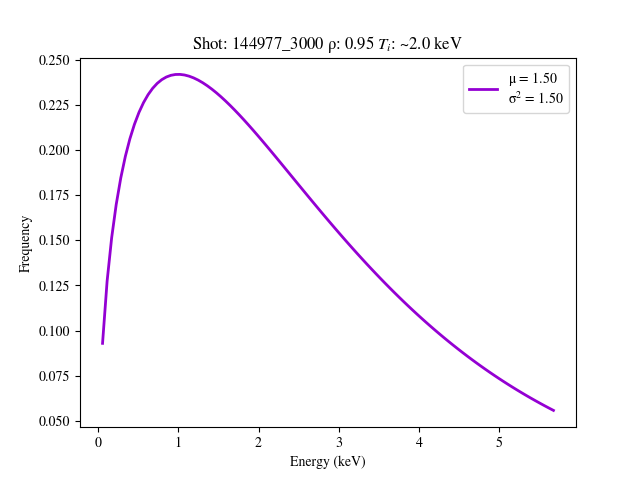
\includegraphics[width=0.5\linewidth]{images/maxwellian_illustration}
		\label{fig:maxwellianGeneral}
	} \quad
	\subfloat[$\rho=0.98$, $T_i=0.517 keV$] {
		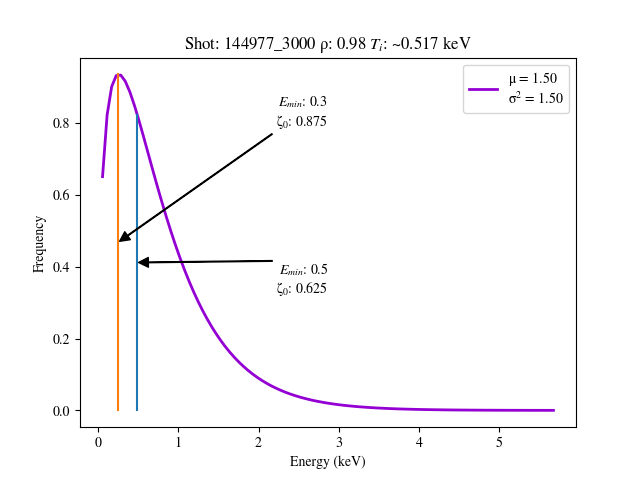
\includegraphics[width=0.5\linewidth]{images/maxwellian_illustration_144977_3000_rho976}
		\label{fig:maxwellianEdge}
	}
	\caption{Maxwellian Gamma Distribution for shot 144977.3000}
\end{figure}

One aspect of the \ac{IOL} that is important to note is that the equilibrium given by \crefrange{eqn:IOLCanonAngleMom}{eqn:IOLMagMom} identify which particles have energy that take them beyond the \ac{LCFS}, but this does not necessarily imply loss. Instead it implies a sufficient orbit to enter unfavorable zones. From this observation, one has to postulate that a certain number of these particles will either i) suffer a collision in the \ac{SOL}, which is not collisionless and therefore reasonable, or ii) particles strike the wall. With this in mind, we utilize the Stacey rational approximation that $R_{loss}^{IOL}$ is approximately 0.5, the logic being that some is more likely than none, while all is probably too much. Half is about right.

\begin{equation}
	F_{rj}^{IOL} \left( r \right) = \cfrac{N_{loss}}{N_{total}} = \cfrac{R_{loss}^{IOL} \bigints_{-1}^{1} \left[ \bigintss_{V_{0,min}}^{\infty} V_0^2 f\left( V_0 \right) dV_0\right] d \zeta_0}{2 \bigintss_{0}^{\infty} V_0^2 f\left(V_0\right)dV_0} = 
	\cfrac{R_{loss}^{IOL} \bigints_{-1}^{1} \BbbGamma \left(\cfrac{3}{2}, \epsilon_{min}\left(\rho,\zeta_0\right)   \right) d\zeta_0}{2 \BbbGamma \left(\cfrac{3}{2}\right)}
	\label{eqn:IOLCumulativeLossParticle}
\end{equation}

\begin{equation}
	M_{rj}^{IOL} \left( r \right) = \cfrac{M_{loss}}{M_{total}} = 
	\cfrac{R_{loss}^{IOL} \bigints_{-1}^{1} \left[ \bigintss_{V_{0,min}}^{\infty} 
		\left(m\,V_0\,\zeta_0\right) V_0^2 f\left( V_0 \right) dV_0\right] d\zeta_0}{2 \bigintss_{0}^{\infty} \left(m\,V_0\right) V_0^2 f\left(V_0\right)dV_0} = 
	\cfrac{R_{loss}^{IOL} \bigints_{-1}^{1} \BbbGamma \left(2, \epsilon_{min}\left(\rho,\zeta_0\right)   \right) d\zeta_0}{2 \BbbGamma \left(2\right)}
	\label{eqn:IOLCumulativeLossMomentum}
\end{equation}


\begin{equation}
	E_{rj}^{IOL} \left( r \right) = \cfrac{E_{loss}}{E_{total}} = \cfrac{R_{loss}^{IOL} \bigints_{-1}^{1} \left[ \bigintss_{V_{0,min}}^{\infty} \left(\cfrac{1}{2} m\,V_0^2\right) V_0^2 f\left( V_0 \right) dV_0\right] d\zeta_0}{2 \bigintss_{0}^{\infty} \left(\cfrac{1}{2} m\,V_0^2\,\zeta_0\right) V_0^2 f\left(V_0\right)dV_0} = 
	\cfrac{R_{loss}^{IOL} \bigints_{-1}^{1} \BbbGamma \left(\cfrac{5}{2}, \epsilon_{min}\left(\rho,\zeta_0\right)   \right) d\zeta_0}{2 \BbbGamma \left(\cfrac{5}{2}\right)} 
	\label{eqn:IOLCumulativeLossEnergy}
\end{equation}


%
%\subsection{Conservation of Momentum} \label{sub:MomentumConservation}

A very important aspect of the equations utilized for this research is that the momentum conservation recovers the fundamental electromagnetic principle inherent in the Lorentz \vxb forces, which are orthogonal to the direction of motion. 
%
\begin{equation}
	\vec{F} = e(\vec{E} + \vxb)
	\label{eqn:Lorentz}
\end{equation}
%
For this reason the bulk fluid toroidal, $V_\varphi$, and poloidal $V_\theta$ velocities influence the radial momentum conservation in \cref{subsub:MCRadial} and the poloidal in \cref{subsub:MCPoloidal}. Additionally, because there is a radial particle flux outward, $\Gamma_{rj},\Gamma_{rk}$, there is a radial electric field that manifests.

\subsubsection{Radial} \label{subsub:MCRadial}
The radial momentum equates the normal force of pressure gradient with the orthogonal contribution of the \vxb. A technique to recapture the pressure is to utilize the gradient scale length (\cref{eqn:GradScalePressure}). It is an empirically derived parameter that is determined from a form of the equations that we are solving \cite{Stacey2004a} and represents a fundamental property in the plasma edge. In the radial direction, the \vxb terms that contribute to the force balance are the $e V_\theta \, B_\varphi$ and the $e$

\begin{equation}
	L_p^{-1} \equiv = \cfrac{1}{p} \diffp{p}r
	\label{eqn:GradScalePressure}
\end{equation}

\begin{equation}
	\begin{bmatrix}
		p_j L^{-1}_{p_j} \\
		p_k L^{-1}_{p_k}
	\end{bmatrix} =
	\begin{bmatrix}
		-\cfrac{1}{1+\cfrac{z_j}{z_k} \cfrac{n_j}{n_k}} & \cfrac{1}{1+\cfrac{z_k}{z_j} \cfrac{n_k}{n_j}} \\
		\cfrac{1}{1+\cfrac{z_k}{z_k} \cfrac{n_j}{n_k}} & -\cfrac{1}{\cfrac{n_k}{n_j} \cfrac{z_k}{z_j}+1}
	\end{bmatrix}^{-1} 
	\begin{bmatrix}
		\cfrac{n_j z_j}{1+\cfrac{n_j}{n_k} \cfrac{m_j}{m_k}} & \cfrac{n_j z_j}{1+\cfrac{n_j}{n_k} \cfrac{m_j}{m_k}} \\
		\cfrac{n_k z_k}{1+\cfrac{n_k}{n_j} \cfrac{m_k}{m_j}} & \cfrac{n_j z_j}{1+\cfrac{n_k}{n_j} \cfrac{m_k}{m_j}}
	\end{bmatrix} 
	\begin{bmatrix}
		e B_\varphi
		\begin{bmatrix}
			V_{\theta j} \\
			V_{\theta k}
		\end{bmatrix} -
		e B_\theta
		\begin{bmatrix}
			V_{\varphi j} \\
			V_{\varphi k}
		\end{bmatrix}
	\end{bmatrix}
	\label{eqn:ConservationOfMomentumRadial}
\end{equation} 


%\begin{multline}
%	\begin{bmatrix}
%		-\cfrac{1}{1+\cfrac{z_j}{z_k} \cfrac{n_j}{n_k}} & \cfrac{1}{1+\cfrac{z_k}{z_j} \cfrac{n_k}{n_j}} \\
%		\cfrac{1}{1+\cfrac{z_k}{z_k} \cfrac{n_j}{n_k}} & -\cfrac{1}{\cfrac{n_k}{n_j} \cfrac{z_k}{z_j}+1}
%	\end{bmatrix} 
%	\begin{bmatrix}
%		p_j L^{-1}_{p_j} \\
%		p_k L^{-1}_{p_k}
%	\end{bmatrix} = \\		
%	\begin{bmatrix}
%		\cfrac{n_j e z_j}{1+\cfrac{n_j}{n_k} \cfrac{m_j}{m_k}} & \cfrac{n_j e z_j}{1+\cfrac{n_j}{n_k} \cfrac{m_j}{m_k}} \\
%		\cfrac{n_k e z_k}{1+\cfrac{n_k}{n_j} \cfrac{m_k}{m_j}} & \cfrac{n_j e z_j}{1+\cfrac{n_k}{n_j} \cfrac{m_k}{m_j}}
%	\end{bmatrix} 
%	B_\phi 
%	\begin{bmatrix}
%		\hat{V}_{\theta_j} \\
%		\hat{V}_{\theta_k}
%	\end{bmatrix} -
%	\begin{bmatrix}
%		\cfrac{n_j e z_j}{1+\cfrac{n_j}{n_k} \cfrac{m_j}{m_k}} & \cfrac{n_j e z_j}{1+\cfrac{n_j}{n_k} \cfrac{m_j}{m_k}} \\
%		\cfrac{n_k e z_k}{1+\cfrac{n_k}{n_j} \cfrac{m_k}{m_j}} & \cfrac{n_j e z_j}{1+\cfrac{n_k}{n_j} \cfrac{m_k}{m_j}}
%	\end{bmatrix} 
%	B_\theta 
%	\begin{bmatrix}
%		\hat{V}_{\phi_j} \\
%		\hat{V}_{\phi_k}
%	\end{bmatrix}
%\end{multline} \label{eqn:ConservationOfMomentumRadial}
\subsubsection{Toroidal} \label{subsub:MCToroidal}

The toroidal momentum balance expressed in \cref{eqn:ConservationMomentumToroidal} equates the forces due to the fluid velocity, $V_\varphi$, with the force due to the toroidal electric field, $E_\varphi^A$, the Lorentz force associated with a radial flux, the momentum input of \ac{NBI} and finally the momentum loss due to \ac{IOL}. It is of some value to deconstruct several of the terms to gain an intuition for these terms.
\begin{itemize}
	\item The force associated with the fluid velocity arises from two physical considerations, collisional drag within the species expressed as a frequency, $\nu_{dj}$, and inter-species drag, $\nu_{jk}$. As an aside it helped the author to do a units analysis that this works to force per unit volume.
	\item The electric field $E_\varphi^A$ is simply a result of current drive and is therefore an externally applied condition.
	\item the $e\,B_\theta \Gamma$ term is a masked Lorentz force. The flux is motion of the charged ionized particles, which produce an orthogonal force as they move across a magnetic field line.
	\item The momentum of the \ac{IOL} term is due to an instantaneous loss of particles. The model description is given in \cref{eqn:IOLCumulativeLossMomentum}
\end{itemize}

\begin{multline}  \label{eqn:ConservationMomentumToroidal}
	\begin{bmatrix}
		n_j m_j \left( \nu_{jk} + \nu^{\varphi}_{dj} \right) & -n_j m_j \nu_{jk} \\
		-n_k m_k \nu_{kj}  & n_k m_k \left( \nu_{kj}+\nu^{\varphi}_{dk} \right)
	\end{bmatrix}
	\begin{bmatrix}
		\hat{V}_{\varphi j}\left(r\right) \\
		\hat{V}_{\varphi k}\left(r\right)								
	\end{bmatrix} = \\
	\begin{bmatrix}
		n_j e_j \\
		n_k e_k
	\end{bmatrix} E^A_{\varphi} +
	\begin{bmatrix}
		e_j B_\theta & 0 \\
		0            & e_k B_\theta
	\end{bmatrix}
	\begin{bmatrix}
		\Gamma_{rj} \left(r\right) \\
		\Gamma_{rk} \left(r\right)
	\end{bmatrix} +
	\begin{bmatrix}
		M_{\varphi j}^\mathrm{nbi}\left(r\right) \\
		M_{\varphi k}^\mathrm{nbi}\left(r\right)
	\end{bmatrix} -
	\begin{bmatrix}
		M_{\varphi j}^\mathrm{iol}\left(r\right) \\
		M_{\varphi k}^\mathrm{iol}\left(r\right)
	\end{bmatrix}
\end{multline}
\subsubsection{Poloidal} \label{subsub:MCPoloidal}

The poloidal momentum conservation is described by \cref{eqn:ConservationOfMomentumPoloidal}. Most of the terms in the poloidal momentum balance are the same as the toroidal momentum balance, which is explained in \cref{subsub:MCToroidal}, but the appropriate changes for the orthogonal Lorentz contributions. The third time on the right of \cref{eqn:ConservationOfMomentumPoloidal}, however, is unique. It results from the gyro-viscous considerations that are negligible in a straight cylindrical plasma, as modeled by Braginskii[\cite{Braginskii1965}], but are significant in a toroidally confined plasma, due to the curvature of the field lines \cite{Stacey2020}. The coefficient, $K$, is the Stacey-Sigmar coefficients which can be found in \citetitle{StaceySigmar1985} \cite{StaceySigmar1985}.

\begin{multline} \label{eqn:ConservationOfMomentumPoloidal}
	\begin{bmatrix}
		n_j m_j \left( \nu_{jk} + \nu^{\theta}_{dj} \right) & -n_j m_j \nu_{jk} \\
		-n_k m_k \nu_{kj}  & n_k m_k \left( \nu_{kj}+\nu^{\theta}_{dk} \right)
	\end{bmatrix}
	\begin{bmatrix}
		\hat{V}_{\theta j}\left(r\right) \\
		\hat{V}_{\theta k}\left(r\right)								
	\end{bmatrix} =
	\begin{bmatrix}
		n_j e_j \\
		n_k e_k
	\end{bmatrix} E^A_{\theta} +
	\begin{bmatrix}
		e_j B_\phi & 0 \\
		0            & e_k B_\phi
	\end{bmatrix}
	\begin{bmatrix}
		\Gamma_{rj} \left(r\right) \\
		\Gamma_{rk} \left(r\right)
	\end{bmatrix} + \\
	\cfrac{B_{\phi}}{B^2}
	\begin{bmatrix}
		\nu^\theta_{dj} \cfrac{K_j}{e_j} & 0 \\
		0 & \nu^\theta_{dk} \cfrac{K_k}{e_k}
	\end{bmatrix}
	\begin{bmatrix}
		L^{-1}_{T_j} \\
		L^{-1}_{T_k}
	\end{bmatrix} +
	\begin{bmatrix}
		M_{\theta j}^\mathrm{nbi}\left(r\right) \\
		M_{\theta k}^\mathrm{nbi}\left(r\right)
	\end{bmatrix} -
	\begin{bmatrix}
		M_{\theta j}^\mathrm{iol}\left(r\right) \\
		M_{\theta k}^\mathrm{iol}\left(r\right)
	\end{bmatrix}
\end{multline}


%
%\subsection{Conservation of Energy} \label{sub:EnergyConservation}

There are conservation considerations for both the primary ion \cref{eqn:EnergyIon} and electron \cref{eqn:EnergyElectron}. Both equations are roughly the same. They are both one-dimensional non-linear radial partial differential equations. There is consideration for beam heating($q_{nbi}$), fast ion orbit loss ($e_{nbi}^{iol}$), and ion-electron ($q_{re}$)  and ion-impurity ($q_{jk}$) cross heating through scattering.  Unique aspects of each are discussed in their subsections. It should be noted that other heat sources can be included, but these are considered the primary heat mechanisms at the moment.

\subsubsection{Ion Radial Heat Flux} \label{subsub:IonRadialHeatFlux}

A unique aspect to the ion radial heat flux (\cref{eqn:EnergyIon}) is that there is consideration for charge exchange, $\langle\sigma v \rangle$ between impurity ions and the primary ion. Also, only the ions experience thermal \ac{IOL}. 

\begin{align} \label{eqn:EnergyIon}
	\cfrac{1}{r}\cfrac{\partial \left(r\hat{Q}_{rj}(r)\right)}{\partial r} = \, q_j^\mathrm{nbi}(r) \left( 1 - \hat{\alpha} e_\mathrm{nbi}^\mathrm{iol}(r) \right) 
	&- q_{je}(r) - q_{jk} \nonumber \\
	&- n_j(r)n_{oj}(r) \langle \sigma v \rangle_\mathrm{cx} \left(\hat{T}_j(r)-T_{oj}\right) -
	\cfrac{\partial E_j^\mathrm{iol}(r)}{\partial r} \hat{Q}_{rj}(r)
\end{align}

\subsubsection{Electron Radial Heat Flux} \label{subsub:ElectronRadialHeatFlux}

For the electron heat equation, there is unique consideration for the radiation emissivity, $L$. 

\begin{multline} \label{eqn:EnergyElectron}
	\cfrac{1}{r}\cfrac{\partial \left(r\hat{Q}_{re}(r)\right)}{\partial r} = q_e^\mathrm{nbi}(r) - q_{je}(r) - q_{ke}  \\
	- n_j(r)n_{oj}(r) \langle \sigma v \rangle_\mathrm{ionj} E_\mathrm{ionj} -
	n_k(r)n_{ok}(r) \langle \sigma v \rangle_\mathrm{ionk} E_\mathrm{ionk} - n_e n_j L_j(r) - n_e n_k L_k(r)
\end{multline}

%
%\subsection{Conduction Closure Equations} \label{sub:ConductionClosure}
As is always the case with the first three moment equations, there is an issue of closure. For this model, we utilize the ion (\cref{eqn:ConductionIon}) and electron conduction (\cref{eqn:ConductionElectron}) closure equations. Both are based on a Fick's law model of heat conduction with a conduction coefficient $\chi$. The radial gradient of heat is proportional to the total heat on sources on the right side. Both models share a total heat term $Q_j, Q_e$ which has been adjusted by a convection like term $\frac{5}{2}T\,\Gamma$, which represents the energy associated with the particles that have been lost. The only unique feature is that the ion conduction equation has a term for the total viscous heat loss and the heat stored in the form of rotation.


\subsubsection{Ion Conduction} \label{subsub:ConductionClosureIon}

\begin{multline} \label{eqn:ConductionIon}
	-n_i \chi_j \left( \cfrac{1}{r} \diffp*{\left( \vphantom{\diffp*{}r}r T_j\left( r \right) \right)}r \right) \equiv	n_j \chi_j T_j(r) L^{-1}_{T_j} = 	q_j\left( r \right) = Q_j \left( r \right) - \cfrac{5}{2} T_j \left( r \right) \Gamma_{rj} \left( r \right) - Q_{\mathrm{vis}_j}(r) - Q_{\mathrm{rot}_j}(r)
\end{multline}

\subsubsection{Electron Conduction} \label{subsub:ConductionClosureElectron}

\begin{equation} \label{eqn:ConductionElectron}
	-n_e \chi_e \left( \cfrac{1}{r} \diffpfunc{r T_e\left( r \right) }{r} \right) \equiv
	n_e \chi_e \func{T_e}{r} L^{-1}_{T_e} = 
	\func{q_e}{r} = \func{Q_e}{r} - \cfrac{5}{2} \func{T_e}{r} \func{\Gamma_{re}}{r}
\end{equation}

%
%\subsubsection{Equilibrium Reconstruction} \label{subsub:EFIT}
A primary input into the \ac{IOL} model is the flux surface $\psi$ (see \cref{eqn:IOLMinV0}). $\psi$ is a parameter that quantifies the amount of enclosed magnetic field. One issue that must determined is the magnetic field topology, both shape and location, which is referred to as MHD equilibrium reconstruction. It is based on solving the Grad-Shafronov equations (\cref{eqn:GradShafDeltaStar} and \cref{eqn:GradShafCurrentDensity}). The work horse tool that performs this reconstruction is EFIT \cite{Lao1990}. It balances the magnetic field forces with toroidal current density, i.e. plasma pressure and Lorentz forces due to poloidal field currents. For this research, the flux surfaces from the MHD reconstruction will be considered as defined.

\begin{equation}
	\Delta \ast \left(\psi\right) = \mu_0 R J_T
	\label{eqn:GradShafDeltaStar}
\end{equation}

\begin{equation}
	J_T = R \left[ P'\left(\psi; \alpha_n\right) + \cfrac{\mu_0 FF' \left(\psi; \gamma_n \right)}{4 \pi^2 R^2}\right]
	\label{eqn:GradShafCurrentDensity}
\end{equation}

%
%\subsection{Beam Modeling} \label{sub:BeamModeling}
The beam model that will be utilized was developed by \citeauthor{Mandrekas1992} \cite{Mandrekas1992} for the "SuperCode". The model is based on a detailed quantum physics analysis to construct the cross-sections, but the implementation was simplified to a fit in \cref{eqn:beamxsection} based on the parameters:
\begin{itemize}
	\item Beam Energy, $E$ in keV/u,
	\item Beam particle atomic number, u
	\item Plasma Z-effective, $Z_{eff}$
	\item Electron Temperature, $T_e$ in keV, and
	\item Ion density, $n_e$ in $\text{cm}^{-3}$.
\end{itemize}
The primary cross-section function, $S_1$, is determined using \cref{eqn:beamS1} and the coefficients \cref{tab:BeamACoefficients}. Similarly, the impurity cross-section function, $S_z$ is calculated \cref{eqn:beamSz} with coefficients being shown in \cref{tab:BeamBCoefficients}. The sensitivity of the cross-section temperature for $Z_{eff}=1$ and $Z_{eff}=2$ are shown in \prettyref{fig:BeamXSecPrimaryTempSweep} and \prettyref{fig:BeamXSecImpurityTempSweep}, respectively. The sensitivity due to density is for the same $Z_{eff}$ are presented in \prettyref{fig:BeamXSecPrimaryDenSweep} and \prettyref{fig:BeamXSecImpurityDenSweep}.

The dominant physics for the beam energies, plasma densities and temperatures for tokamak plasmas are collisional radiative \cite{Janev1989}. 


\begin{equation}
	\sigma_s^{\left(z\right)}\left(E, n_e, T_e, Z_{eff}\right) = \cfrac{\exp\left[S_1\left(E, n_e, T_e\right)\right]}{E}
	\times \left[1 + \left(Z_{eff}-1\right) S_z\left(E, n_e, T_e\right) \right] \left(\times 10^{-16} \text{cm}^2 \right)
	\label{eqn:beamxsection}
\end{equation}
%
where
%
\begin{equation}
	S_1 = \sum_{i=1}^{2} \sum_{j=1}^{3} \sum_{k=1}^{2} \left\{ A_{ijk} \times \left(\ln E\right)^{i-1} 
	\left[ \ln \left(\cfrac{n}{n_0}\right) \right]^{j-1} \left( \ln T_e\right)^{k-1} \right\}
	\label{eqn:beamS1}
\end{equation}
%
and
%
\begin{equation}
	S_z = \sum_{i=1}^{3} \sum_{j=1}^{2} \sum_{k=1}^{2} \left\{ B_{ijk}^{\left(z\right)} \times \left(\ln E\right)^{i-1} 
	\left[ \ln \left(\cfrac{n}{n_0}\right) \right]^{j-1} \left( \ln T_e\right)^{k-1} \right\}
	\label{eqn:beamSz}
\end{equation}

\begin{table}
	\centering
	\caption{Values of fit coefficients\cite{Janev1989}}
	\subfloat[$A_{ijk}$ coefficients \newline \cref{eqn:beamS1}] {
		\begin{tabular}{|l|l|}
			\hline
			$ A_{ijk} $ &                                     \\
			\hline
			$ A_{111} $ & $\hphantom{-}4.40                $  \\
			$ A_{112} $ & $           -2.49 \times 10^{-2} $  \\ 
			$ A_{121} $ & $\hphantom{-}7.46 \times 10^{-2} $  \\ 
			$ A_{122} $ & $\hphantom{-}2.27 \times 10^{-3} $  \\ 
			$ A_{131} $ & $\hphantom{-}3.16 \times 10^{-3} $  \\ 
			$ A_{132} $ & $           -2.78 \times 10^{-5} $  \\
			$ A_{211} $ & $\hphantom{-}2.30 \times 10^{-1} $  \\
			$ A_{212} $ & $           -1.15 \times 10^{-2} $  \\
			$ A_{221} $ & $           -2.55 \times 10^{-3} $  \\
			$ A_{222} $ & $           -6.20 \times 10^{-4} $  \\
			$ A_{231} $ & $           -1.32 \times 10^{-3} $  \\
			\hline
		\end{tabular}	
		\label{tab:BeamACoefficients}
	} \quad
	\subfloat[$B_{ijk}$ coefficients for He, C, O and Fe Impurities \newline \cref{eqn:beamSz}] {
		\begin{tabular}{|l|c|c|c|c|}
			\hline
			$ B_{ijk}^{\left(z\right)}$ & He & C &  O & Fe \\
			\hline
			$ B_{111} $ & $           -2.36 \times 10^{0\hphantom{-}} $  
			            & $           -1.49 \times 10^{0\hphantom{-}} $ 
			            & $           -1.41 \times 10^{0\hphantom{-}} $ 
			            & $           -1.03 \times 10^{0\hphantom{-}} $ \\
			$ B_{112} $ & $\hphantom{-}1.85 \times 10^{-1} $  & $           -1.54 \times 10^{-2} $ &  $           -4.08 \times 10^{-4} $ & $\hphantom{-}1.06 \times 10^{-1} $ \\
			$ B_{121} $ & $           -2.50 \times 10^{-1} $  & $           -1.19 \times 10^{-1} $ &  $           -1.08 \times 10^{-1} $ & $           -5.58 \times 10^{-2} $ \\
			$ B_{122} $ & $           -3.81 \times 10^{-2} $  & $           -1.50 \times 10^{-2} $ &  $           -1.38 \times 10^{-2} $ & $           -3.72 \times 10^{-3} $ \\
			$ B_{211} $ & $\hphantom{-}8.49 \times 10^{-1} $  & $\hphantom{-}5.18 \times 10^{-1} $ &  $\hphantom{-}4.77 \times 10^{-1} $ & $\hphantom{-}3.22 \times 10^{-1} $ \\
			$ B_{212} $ & $           -4.78 \times 10^{-2} $  & $\hphantom{-}7.18 \times 10^{-3} $ &  $\hphantom{-}1.57 \times 10^{-3} $ & $           -3.75 \times 10^{-2} $ \\
			$ B_{221} $ & $\hphantom{-}6.77 \times 10^{-2} $  & $\hphantom{-}2.92 \times 10^{-2} $ &  $\hphantom{-}2.59 \times 10^{-2} $ & $\hphantom{-}1.24 \times 10^{-2} $ \\
			$ B_{222} $ & $\hphantom{-}1.05 \times 10^{-2} $  & $\hphantom{-}3.66 \times 10^{-3} $ &  $\hphantom{-}3.33 \times 10^{-3} $ & $\hphantom{-}8.61 \times 10^{-4} $ \\
			$ B_{311} $ & $           -5.88 \times 10^{-2} $  & $           -3.36 \times 10^{-2} $ &  $           -3.05 \times 10^{-2} $ & $           -1.87 \times 10^{-2} $ \\
			$ B_{312} $ & $\hphantom{-}4.34 \times 10^{-3} $  & $\hphantom{-}3.41 \times 10^{-4} $ &  $\hphantom{-}7.35 \times 10^{-4} $ & $\hphantom{-}3.53 \times 10^{-3} $ \\
			$ B_{321} $ & $           -4.48 \times 10^{-3} $  & $           -1.79 \times 10^{-3} $ &  $           -1.57 \times 10^{-3} $ & $           -7.43 \times 10^{-4} $ \\
			$ B_{322} $ & $           -6.76 \times 10^{-4} $  & $           -2.04 \times 10^{-4} $ &  $           -1.86 \times 10^{-4} $ & $           -5.12 \times 10^{-5} $ \\
			\hline
		\end{tabular}	
		\label{tab:BeamBCoefficients}
	}
\end{table}

\begin{figure}[!ht]
	\subfloat[$ Z_{eff} = 1 $] {
		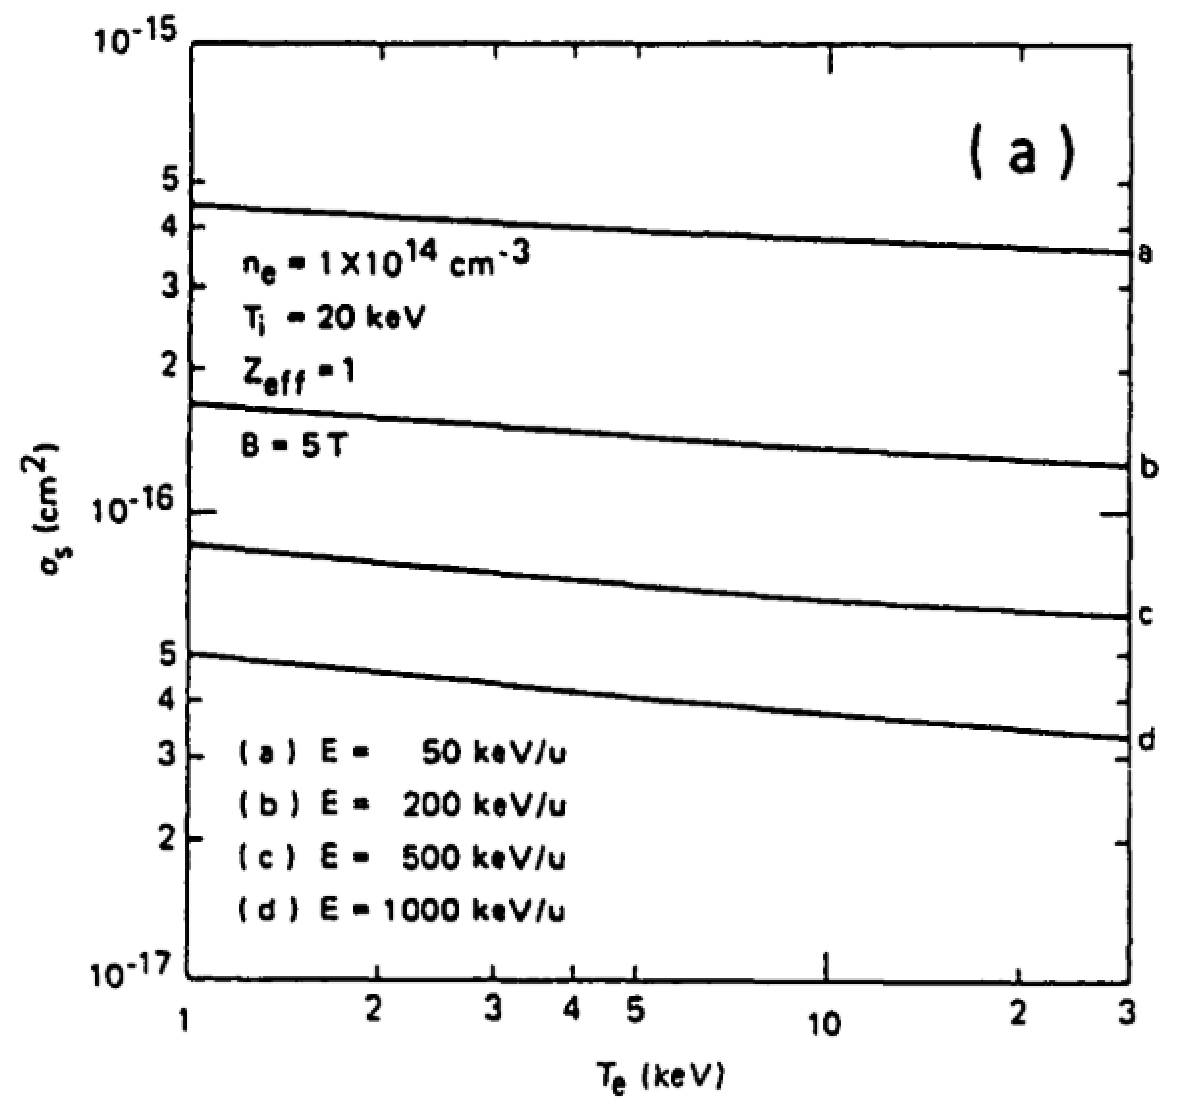
\includegraphics[width=0.45\linewidth]{images/beam_xsec_primary_temp_sweep}
		\label{fig:BeamXSecPrimaryTempSweep}
	} \quad
	\subfloat[$ Z_{eff} =2 $] {
		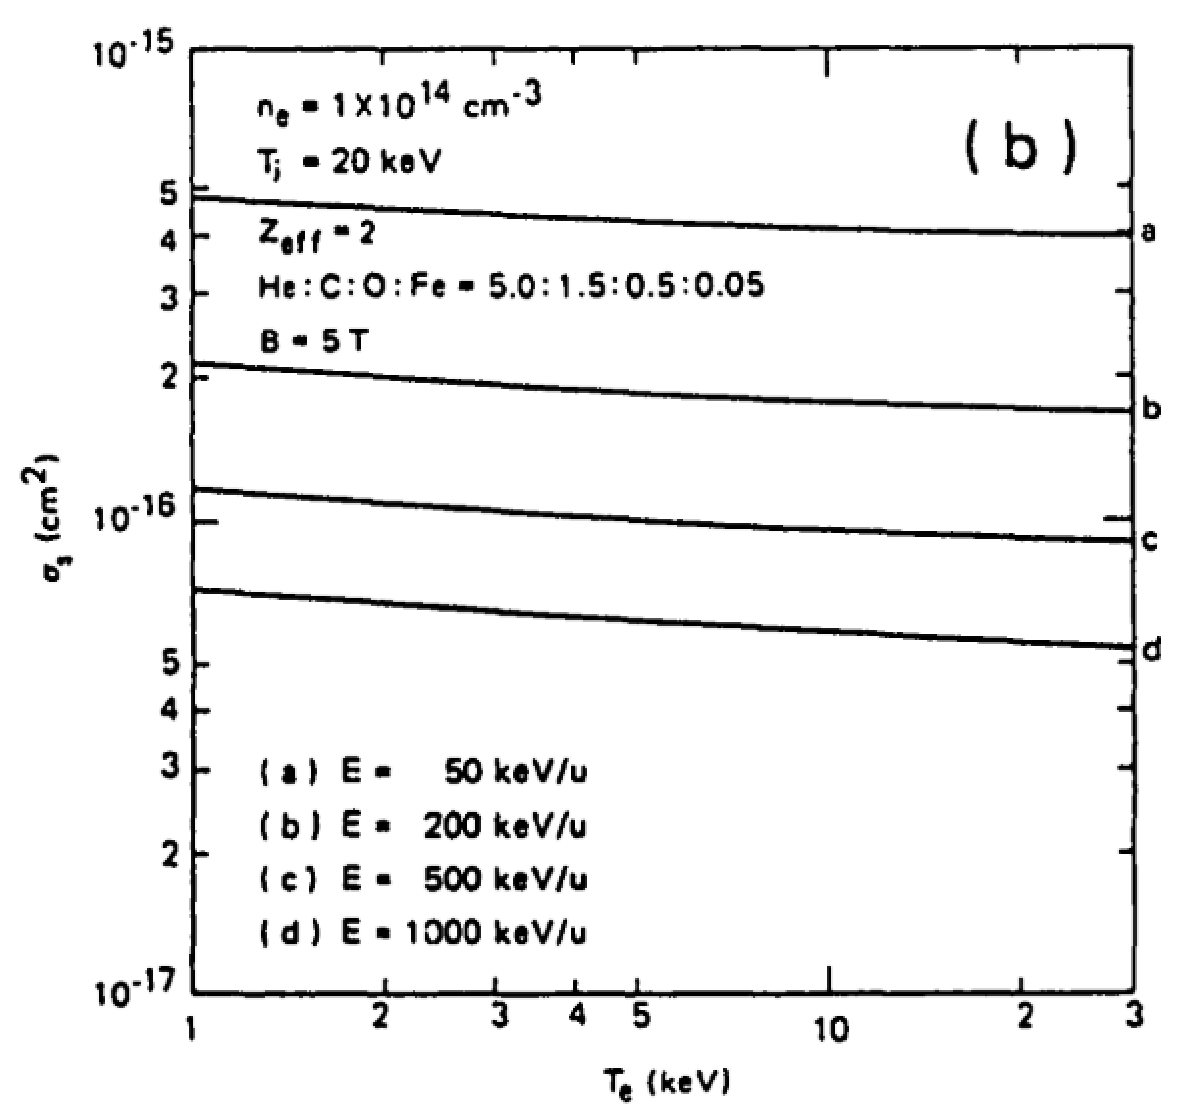
\includegraphics[width=0.45\linewidth]{images/beam_xsec_impurity_temp_sweep}
		\label{fig:BeamXSecImpurityTempSweep}
	}
	\caption{Temperature dependence of $\sigma_s$ for $n_e = 10^{14} \text{ cm}^{-3}$ for several beam energies \cite{Janev1989}}
\end{figure}


\begin{figure}[!ht]
	\subfloat[$ Z_{eff} = 1 $] {
		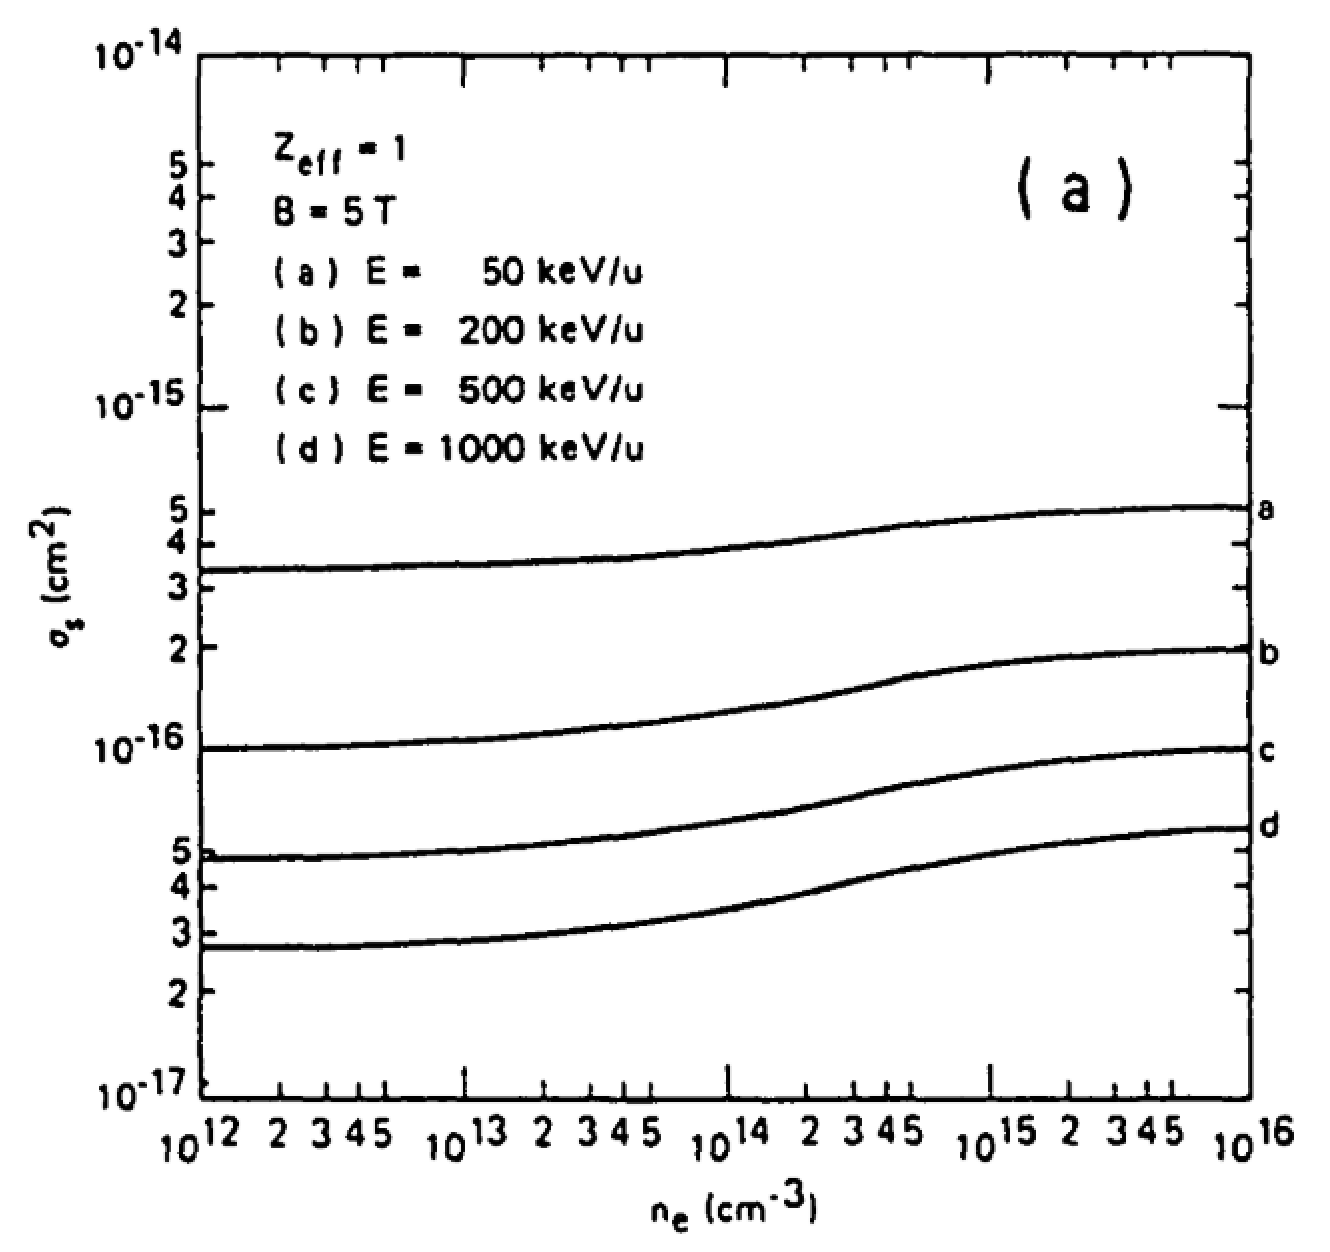
\includegraphics[width=0.45\linewidth]{images/beam_xsec_primary_den_sweep}
		\label{fig:BeamXSecPrimaryDenSweep}
	} \quad
	\subfloat[$ Z_{eff} =2 $] {
		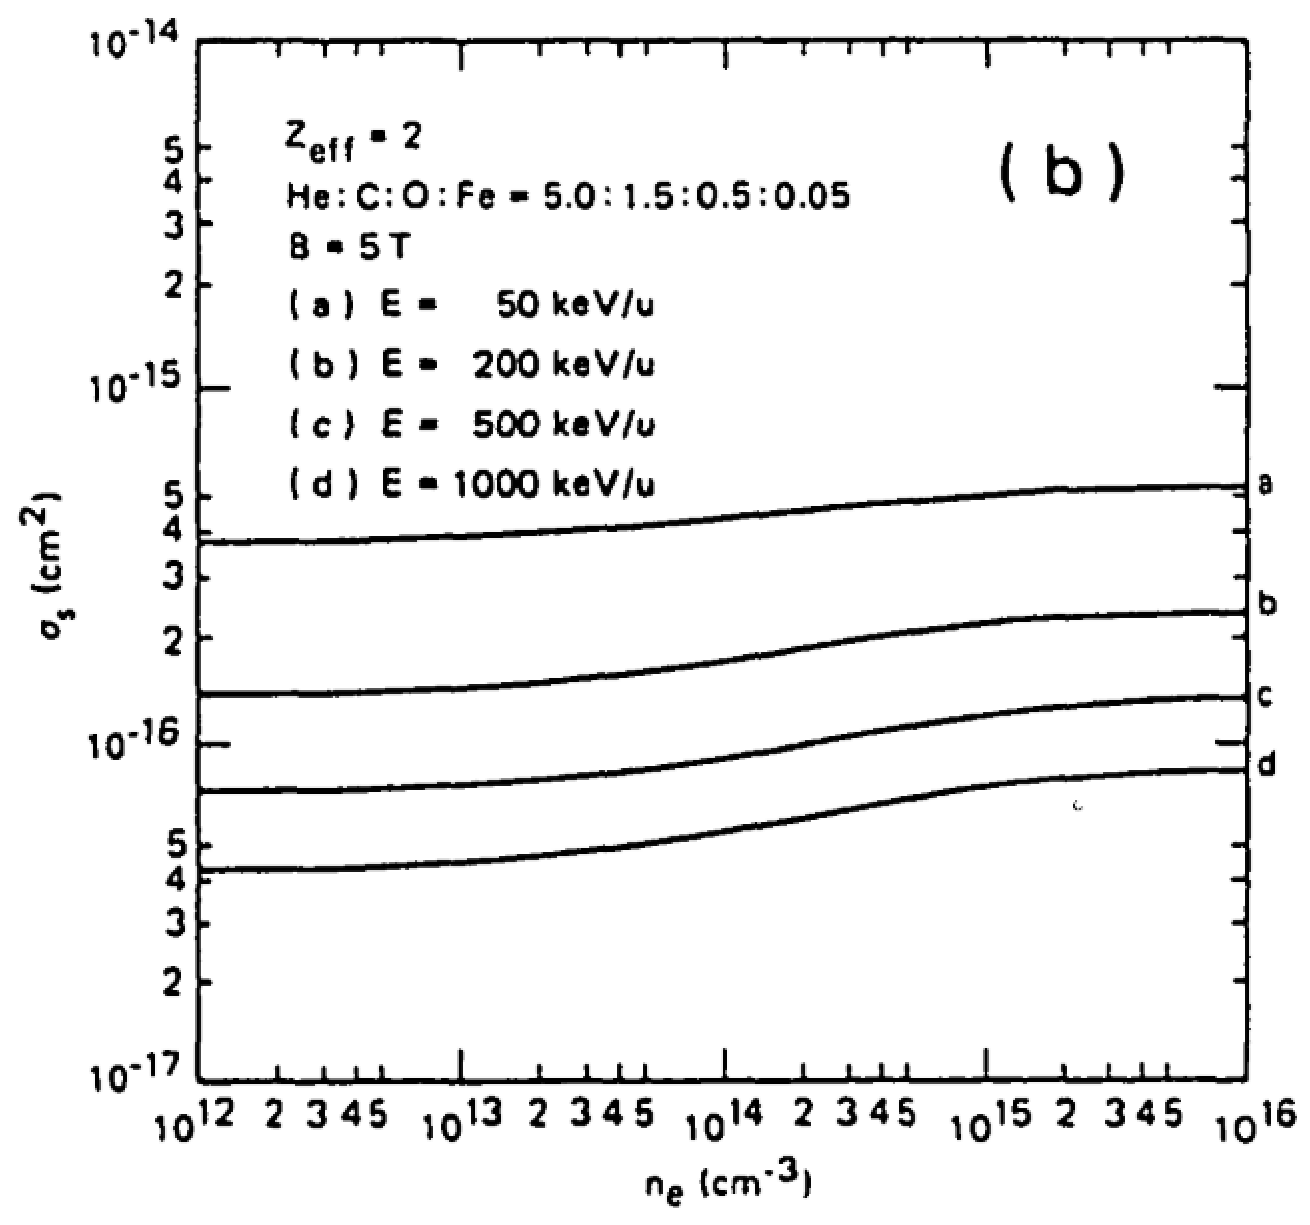
\includegraphics[width=0.45\linewidth]{images/beam_xsec_impurity_den_sweep}
		\label{fig:BeamXSecImpurityDenSweep}
	}
	\caption{Density dependence of $\sigma_s$ for several beam energies \cite{Janev1989}}
\end{figure}
%
%%\subsection{Ionization Modeling}\label{sub:Ionization}
%
%\subsection{Ideal Gas Law}\label{sub:IdealGasLaw}
%
%The relationship between the pressure calculated in the momentum equation and the density that initializes the iteration, there is an implied temperature which is given by the ideal gas law
%\begin{equation}
%	P = n\, T
%	\label{eqn:IdealGasLaw}
%\end{equation}
%Based on the iteration strategy chosen (\cref{sec:ComputationalModeling}), this temperature must align with the temperature implied by conservation of energy.
%
%\subsection{Pinch Diffusion} \label{sub:PinchDiffusion}

It is hoped that this research will culminate with an easy way to reincorporate the \vxb and \ac{IOL} physics into traditional diffusion models. In \cite{Stacey2019}, \citeauthor{Stacey2019} provides a diffusion-like model that has a $\Gamma^{Pinch}$ term that retains the \vxb and \ac{IOL}. $\Gamma^{Pinch}$, which appears in \cref{eqn:PinchDiffusion}, is given by the expression in \cref{eqn:PinchDiffusionFlux}.

\begin{equation}
	\diffp*{\left( D_{jj} \diffp{n_j}r \right)  }r - \diffp*{\left( D_{jk} \diffp{n_k}r \right)  }r - \diffp*{\left( D_{jj} \frac{n_j}{T_j}\diffp{T_j}r \right)  }r -\diffp*{\left( D_{jk} \frac{n_j}{T_k}\diffp{T_k}r \right)  }r + \diffp{\Gamma_{rj}^{pinch}}r = S_j
	\label{eqn:PinchDiffusion}
\end{equation}

\begin{equation}
	\Gamma_{rj}^{pinch} \equiv - \cfrac{n_j E_\phi^A}{B_\theta} - \cfrac{M_{\phi j}}{e_j B_\theta} + 
	\cfrac{n_j m_j \left( \nu_{jk} + \nu_{dj} \right) }{e_j B_\theta} 
	\left( \cfrac{E_r}{B_\theta} + \cfrac{B_\phi}{B_\theta} V_{\phi j} \right)
	- n_j m_j \nu_{jk} V_{\phi k}	
	\label{eqn:PinchDiffusionFlux}
\end{equation}
%
The diffusion coefficients embed the drag frequency, $\nu_{dj}$, and the inter-species collisional frequency $\nu_{jk}$.
%
\begin{equation}
		D_{jj} \equiv \cfrac{m_j T_j \left( \nu_{dj} + \nu_{jk} \right) }{\left(  e_j B_\theta \right)^2}, \quad
		D_{jk} \equiv \cfrac{m_j T_j \nu_{jk} }{ e_j e_k B_\theta^2}
		\label{eqn:PinchDiffusionCoefficients}
\end{equation}

%
%\subsection{Neutral Transport} \label{sub:NeutralTransport}

Neutrals from gas injection and gas recycling from the wall are:

\begin{itemize}
	\item ionized by interaction with electrons, which produces 
	\begin{itemize}
		\item a plasma ion in the ion particle balance equation \cref{eqn:Continuity} and
		\item an ionization cooling term in the ion energy balance equation \cref{eqn:EnergyIon}; and
	\end{itemize}
%
	\item interacts with a plasma ion to effectively replace a hot ion with a cool ion ( charge exchange cooling term in the ion energy balance equation \cref{eqn:EnergyIon}).
\end{itemize}

The transport of these neutrals are modeled using \acf{TEP} methodology \cite{Stacey1994, Stacey2000a, Stacey2001b, Rubilar2001, Stacey2001c, Mandrekas2003, Zhang2006}. The \ac{TEP} physics are based on a probabilistic description of interacting and transmitting particles within a region of interest (i). The partial current, $J_{ij}$ from a region i (note this is not indicating ions) to region j is described by \cref{eqn:GTneutPartialCurrent}.

\begin{equation}
	J_{ij} = \sum_{k}^{k}J_{ki}T_{0i}^{ku} + \sum_{k}^{i}\left(1-\sum_{l}^{i}T_{0i}^{kl}\right) J_{ki} c_i P_i \Lambda_{ij} + s_i P_i \Lambda{ij}^s
	\label{eqn:GTneutPartialCurrent}
\end{equation}

The first term accounts for all of the partial currents entering region i (see \prettyref{fig:tepschematic}) from all contiguous region k that transmit through region i. This is found by multiplying edge currents, $J_{ki}$ by the transmission probability $T_{0i}^{kj}$. The second term represents all of the partial currents entering region i from contiguous regions that suffer a collision inside of region i. The collision probability is $c_i$, the escape probability is, $P_i$ and the probability that scattered particles from region i escape to region j $\Lambda_{ij}$. The third term represents any internal source, such as recombination. Further description can be found in Section 2 of \citeauthor{Rubilar2001} \cite{Rubilar2001}.


\begin{figure}
	\centering
	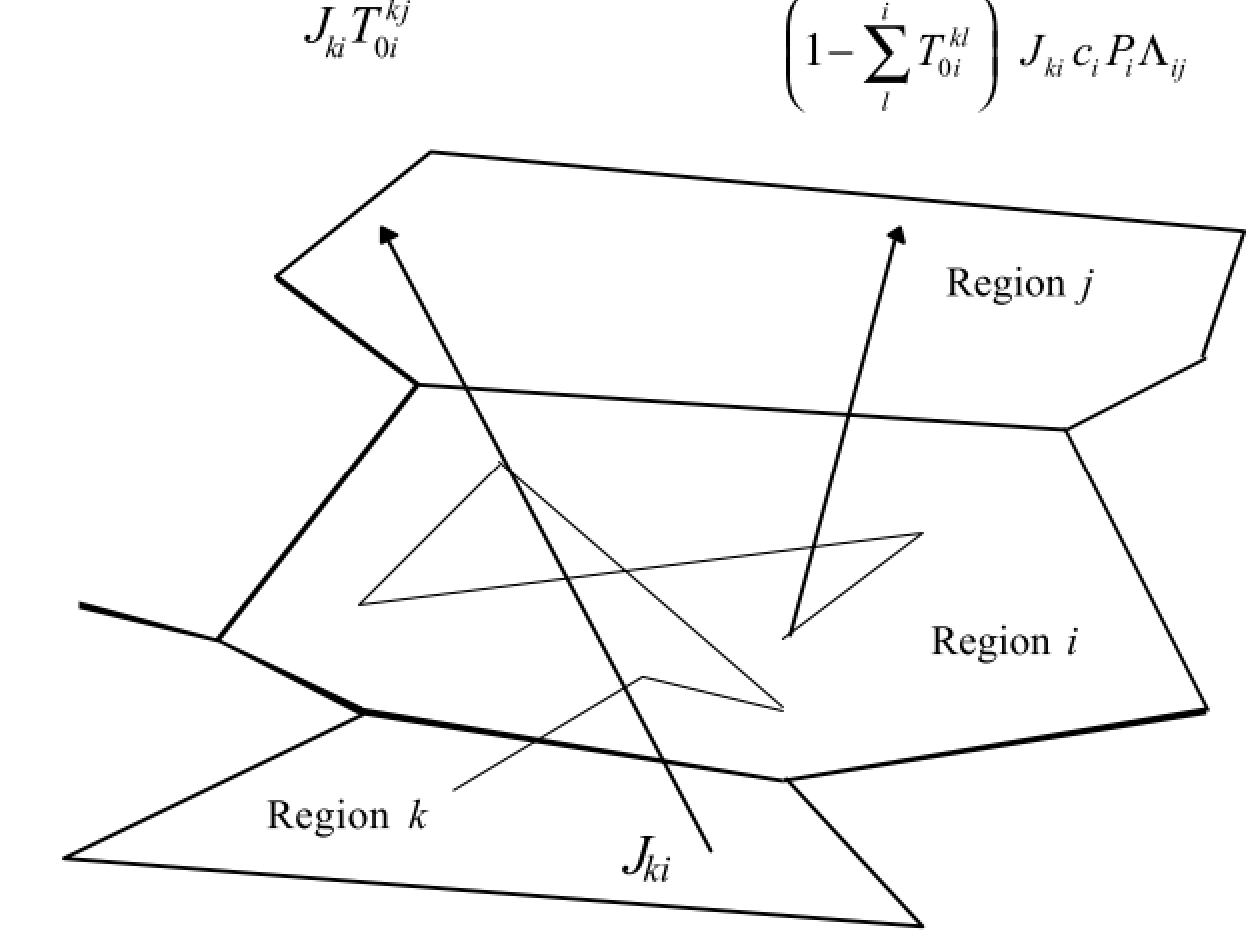
\includegraphics[width=0.7\linewidth]{images/TEP_schematic}
	\caption[TEP]{\acf{TEP} schematic diagram in 2-D geometry \cite{Rubilar2001}}
	\label{fig:tepschematic}
\end{figure}

For our purposes, it has been suggested that a simplified neutral transport implementation from \citeauthor{Stacey2000a} \citeyear{Stacey2000a} \cite{Stacey2000a}, utilizing GTNeut, should suffice. The simplified model breaks the plasma into regions shown in \prettyref{fig:gtneutschematic}. This modeling approach will be utilized initially and modified as needed.

\begin{figure}
	\centering
	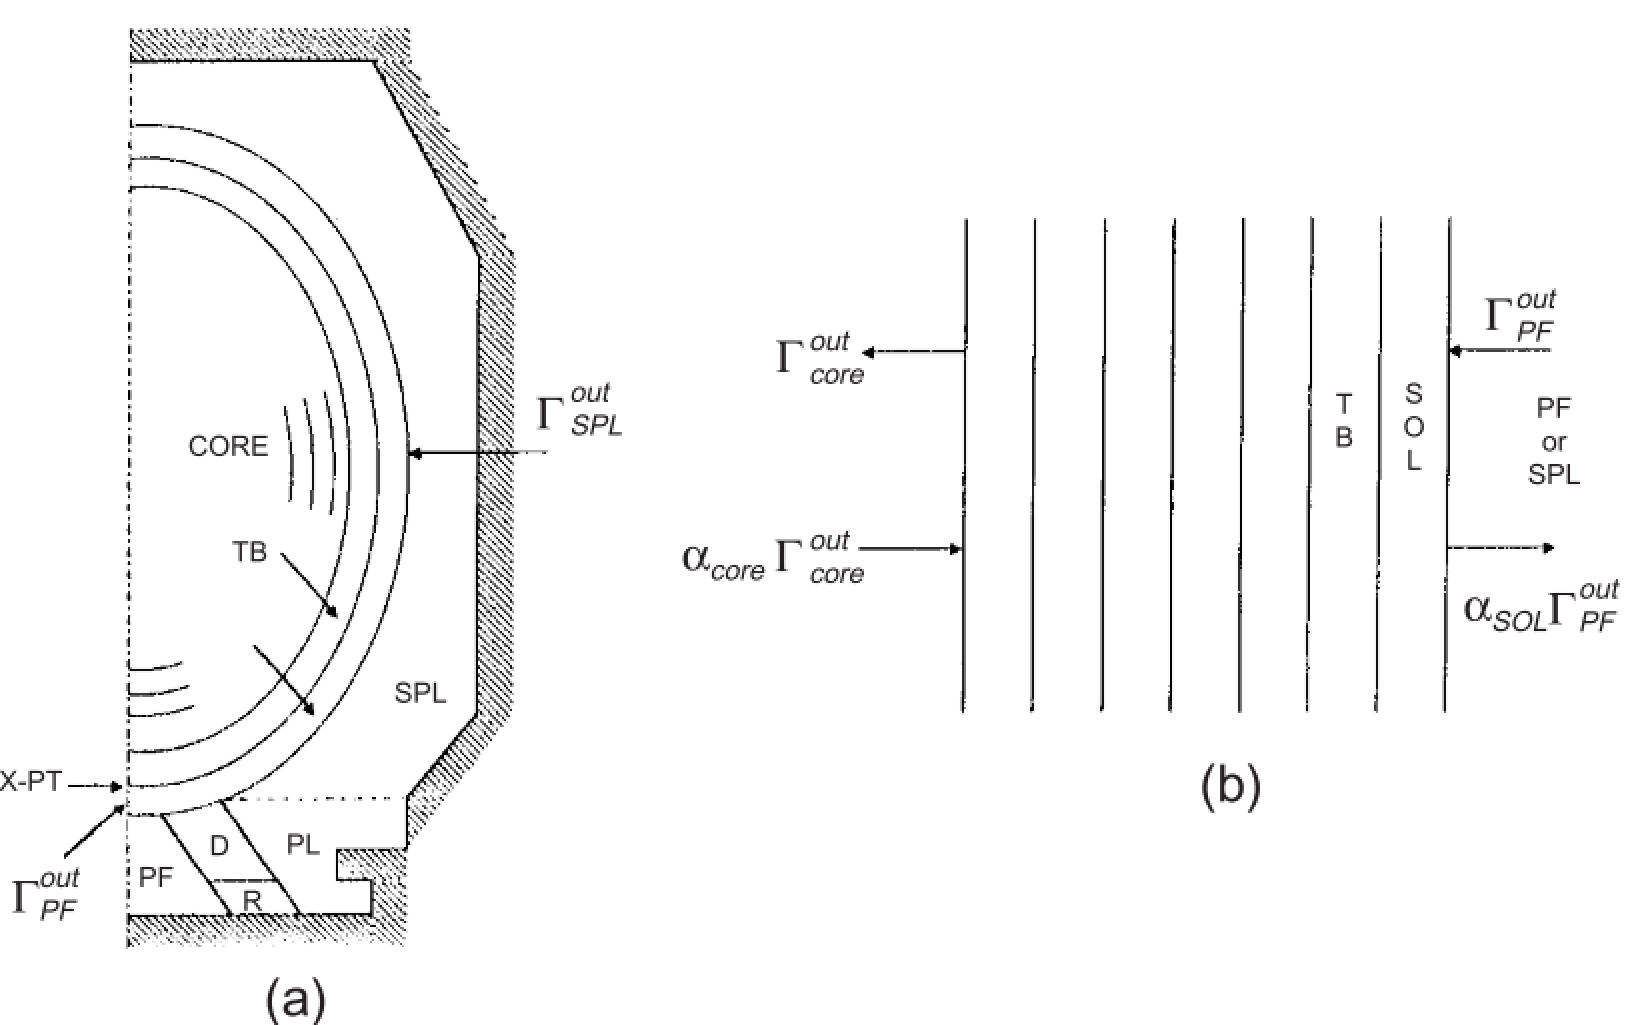
\includegraphics[width=0.7\linewidth]{images/GTNeut_schematic}
	\caption[GTNeutSchematic]{Schematic diagram of the neutral transport model: (a) 2-D TEP model of divertor plasma (D), recycling region (R), private flux (PF), plenum (PL) and SOL plenum (SPL); (b) 1-D ICB model of penetration through SOL and transport barrier (TB) into core. \cite{Stacey2000a}}
	\label{fig:gtneutschematic}
\end{figure}




\section{Computational Modeling}\label{sec:ComputationalModeling}

Identifying the appropriate computational approach to solving a system of equations begins with a characterization of the equations. Often this can be a daunting exercise for complex models and sub-models, as is the case with this problem. The first observation about our system of equations is that they all are one dimensional in the radial direction except for the \ac{IOL} model. \ac{IOL} necessarily requires a poloidal consideration, which makes this model a 1.5 dimensional model. From there, the equations generally fall into two categories, either partial first order, non-linear, differential equations or algebraic. \prettyref{tab:DiffEqCategorization} shows the differential equations and their categorization while \prettyref{tab:AlgebraicCategorization} lists the algebraic ones. Because the equations are non-linear, the solution algorithms must be iterative in nature. The primary solver that will be explored is the Broyden solver, which is a variant within the family of Newton-Raphson solvers. The solver is discussed in \prettyref{sub:SolverSelection}.

\renewcommand\arraystretch{1.5}
\newcolumntype{L}[1]{>{\raggedright\arraybackslash}m{#1}}
\newcolumntype{C}[1]{>{\centering\arraybackslash}m{#1}}
\newcolumntype{R}[1]{>{\raggedleft\arraybackslash}m{#1}}

\begin{table}
\centering
\caption{Categorization of Differential Equations}
\begin{tabular}{|L{0.2\linewidth}|C{0.1\linewidth}|c|c|p{0.35\linewidth}|}
	\hline
	Equation & Number &Order & Type & Reason \\
	\hline
	Particle Conservation & \ref{eqn:Continuity} & 1st & Non-linear & \ac{IOL} Coefficient on $\Gamma$ is a function of $\Gamma$ vicariously through the Temperature \\
	\hline
	Energy & \ref{eqn:EnergyIon} \& \ref{eqn:EnergyElectron} & 1st & Non-linear & \ac{IOL} Coefficient on $\Gamma$ is a function of $\Gamma$ vicariously through the Temperature \\
	\hline
	Conduction Closure & \ref{eqn:ConductionIon} \& \ref{eqn:ConductionElectron} & 1st & Non-linear & Temperature multiplied by $\Gamma$ \\
	\hline
\end{tabular}
\label{tab:DiffEqCategorization}
\end{table}

\begin{table}
	\centering
	\caption{List of Algebraic Equations}
	\begin{tabular}{|l|c|}
		\hline
		Equation & Number \\
		\hline
		Minimum Energy & \ref{eqn:IOLMinV0} \& \ref{eqn:IOLEmin} \\
		\hline
		Radial Momentum & \ref{eqn:ConservationOfMomentumRadial} \\
		\hline
		Toroidal Momentum & \ref{eqn:ConservationMomentumToroidal} \\
		\hline
		Poloidal Momentum & \ref{eqn:ConservationOfMomentumPoloidal} \\
		\hline
		Beam Cross-section & \ref{eqn:beamxsection} \\
		\hline
	\end{tabular}
	\label{tab:AlgebraicCategorization}
\end{table}

\subsection{Iteration Strategy} \label{sub:CalculationOrder}

The iteration strategy requires that consideration be made for calculation order. Identifying what parameters to initialize and which ones to solve for require thought. From the initial guessed parameters, the sequence of calculations should progress in such a way that all subsequent equations have the necessary input to avoid the nefarious "use-before-calculate". The flow chart in \prettyref{fig:flowchart} shows the iteration strategy chosen. The easiest way to understand the chart is to begin with the error term $\Delta T_i$. Essentially, there are two manners by which to arrive at the ion temperature. The upper half of the flow-map utilizes an initial guess of densities, both primary ion and impurity as well as electron temperature, to source the conservation of momentum and the Beam Cross-section/Deposition calculations. Combining these with the results of the Particle conservation results in a calculation of pressure which then implies a temperature through the ideal gas law.

The second path on the lower half of the flow chart determines a temperature by way of a thermal \ac{IOL} and a fast \ac{IOL} calculation, which then feeds the conservation of energy and conduction closure equations. This results in a separate temperature. The iteration then proceeds from the error in ion temperature. The solver, of which ever flavor eventually chosen, must intelligently update the primary ion density until a solution is found.

The impurity density in this iteration strategy is assumed to be specified, since this study does not consider mechanisms of impurity source generation.

It is also worth noting that the conservation of momentum calculation was ordered the way that it is, because the poloidal and toroidal momentum equations have:
\begin{itemize}
	\item calculated particle flux, $\Gamma$ from particle conservation, 
	\item toroidal $E_\varphi^A$ and poloidal $E_\theta^A$ electric fields, which are user specified,
	\item calculated \ac{IOL} momentum contributions, and
	\item user specified \ac{NBI} momentum contributions
\end{itemize}

\begin{sidewaysfigure}[ht]
	\centering
	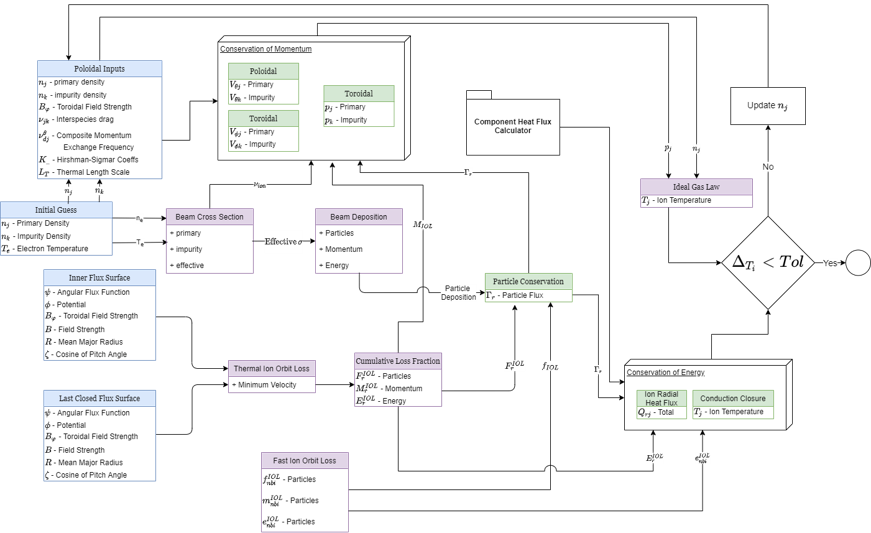
\includegraphics[width=\textwidth]{images/IterationFlowChart}
	\caption[Flow Chart]{Iteration Strategy Flow Chart}
	\label{fig:flowchart}
\end{sidewaysfigure}

\subsection{Solver Selection} \label{sub:SolverSelection}

Algebraic solvers, such as Gauss-Jordan reduction, are applicable to predictive calculations where the densities and temperatures are sourced by experimental data, but they are not applicable to boundary valued iterative problems. 
Of the solvers that appropriate for iterative techniques, several but were considered and dismissed. \acf{GMRES} style solvers are appropriate for a non-symmetric system of linear equations \cite{Kelley1995}. Our equations are non-linear. Pure Newton Methods were dismissed because they require analytic functions so that the Jacobian can be analytically calculated. Our equations do not have an obvious analytic form. That leaves us with quasi Newton-Raphson methods in which the Jacobian is calculated computationally. The most widely used quasi Newton-Raphson method is the Broyden method. The Broyden method approaches the rate of convergence of a pure Newton-Raphson method, however, it accomplishes this at a fraction of the computational cost because the full Jacobian is not recalculated, but is evaluated numerically and algorithmically updated in subsequent iterations.

The update of values from iteration to iteration follows a similar approach to Newton's methods (\cref{eqn:BroydenUpdate}), namely:
%
\begin{equation}
	x_{+} = x_c - B_c^{-1} F(x_c).
	\label{eqn:BroydenUpdate}
\end{equation}
%
This nomenclature is directly borrow from reference \cite{Kelley1995}. The subscript c indicates current values, whereas the + refers to updated values. F is the function being evaluated, and B is the Broyden matrix which is the numerical analogue of the analytic Jacobian. In pure Newton's methods, the Jacobian would be recalculated for each successive iteration. However, Broyden's method utilizes a secant update approach given by \cref{eqn:BroydenSecant}

\begin{equation}  \label{eqn:BroydenSecant}
	\begin{split}
		B_{+} = B_c + \cfrac{\left(y - B_c \, s) s^T\right)}{s^T s} = B_c + \cfrac{F(x_{+})s^T}{s^Ts} \\
		\text{where } y = F(x_{+}) - F(x_c) \text{ and } s = x_{+} - x_c
	\end{split}
\end{equation}

One last thing should be noted. It is unknown at this point how non-linear the system of equations are. If the \ac{IOL} proves to not be sensitive to changes in temperature, then it might be possible to revisit other iterative techniques such as \ac{GMRES}.



\section{Validation}\label{sec:ValidationStrategy}

Dimensional Analysis \cite{Buckingham1914} is a powerful tool for understanding and interpreting key characteristics in the experimental data. Similitude, the science of characterizing a physical system using a scale invariant parameter space, has been a workhorse in aerodynamics, especially wind tunnel experiments, and is required by the ITER Physics Expert Group for Confinement and Transport for plasma test facilities to demonstrate ITER relevant experiments \cite{Connor1977}. The advantage of similitude in an experimental context is that a tokamak of smaller scale can achieve plasma dynamically similar conditions to ITER. A subtlety that is often overlooked is the value of dimensional analysis when conducting a model validation. The intent of our research is to apply the techniques of Buckingham $\Pi$ Theorem to identify the dimensionless groups embedded in our set of equations, reduce the experimental data according to these dimensionless groups and do a model comparison against this data in this non-dimensional space.

\subsection{Dimensional Analysis} \label{sub:DimensionalAnalysis}

The objective of dimensional analysis is to represent the physics of a system in a scale invariant parameter space. The methodology to reduce a system in such a way had a history of being utilized in earlier work, was formalized by \citeauthor{Buckingham1914} in his paper \citetitle{Buckingham1914} in \citeyear{Buckingham1914} \cite{Buckingham1914}. The methodology to produce the scale invariant parameters, known as dimensionless groups, is outlined in \prettyref{subsub:BuckinghamPiTheorem}.

The result of applying the Buckingham approach is a set of dimensionless groups 

\subsubsection{Dimensionless Groups and the Buckingham Theorem} \label{subsub:BuckinghamPiTheorem}

\subsubsection{Application Similarity} \label{subsub:Similarity}

\subsection{}


The model must be validated against a variety of plasma modes. The parameters of interest include both carbon and electron densities and temperatures, as well as rotation velocities/frequencies. Some of the important modes to consider include:

\begin{itemize}
	\item \gls{L-Mode},
	\item \gls{H-Mode},
	\item \gls{SH-Mode},
	\item \ac{RMP}, and
	\item \gls{NT-Mode}
\end{itemize}

Test data showing various profiles have been presented to illustrate some of the differences in profile behavior that needs to be modeled. 
Carbon and electron temperature are illustrated in \prettyref{fig:TestDataCarbonTemp} and \prettyref{fig:TestDataElectronTemp}, respectively, while their densities are shown in \prettyref{fig:TestDataCarbonDensity} and \prettyref{fig:TestDataElectronDensity}, respectively. Finally, available rotation data for several shots are presented in \prettyref{fig:TestDataToroidalRotation}. Some shots show steep gradients while others less so. Rather than presenting a detailed comparison of features in the presented data set, what is relevant for this research is that hope of this methodology is to successfully reproduce curvatures and gradients exhibited in the test data.

\begin{table}
	\centering
	\caption{Some Selected Shots for Validation}
	\begin{tabular}{|c|c|c|}
		\hline
		Shot Type & Shot Number & Time (ms) \\
		\hline
		L-Mode & 144567 & 4000 \\
		\hline
		H-Mode & 161409 & 5000 \\
		\hline
		SH-Mode & 171322 & 1800 \\
		\hline
		RMP & 161409 & 5600 \\
		\hline
		NT-Mode & 179990 & 1400 \\
		\hline
	\end{tabular}
	\label{tab:SelectedShots}
\end{table}

\clearpage

%\newcommand{\Lshot}{144567\_4000}
%\newcommand{\Hshot}{161409\_5000}
%\newcommand{\SHshot}{171322\_1800}
%\newcommand{\RMPshot}{161409\_5600}
%\newcommand{\NTshot}{179990\_1400}
\newcommand{\figdim}{0.45\linewidth}

\newcommand{\figdata}{carbon_temperature}

\begin{figure}
	\centering
	\subfloat[L-Mode 144567\_4000]{
		\includegraphics[width=\figdim]{images/testdata/144567_4000_\figdata}
	}
	\subfloat[H-Mode Shot:161409\_5000]{
		\includegraphics[width=\figdim]{images/testdata/161409_5000_\figdata}
	} \\
	\hspace{0mm}
	\subfloat[SH-Mode Shot:171322\_1800]{
		\includegraphics[width=\figdim]{images/testdata/171322_1800_SH_\figdata}
	}
	\subfloat[RMP Shot:161409\_5600]{
		\includegraphics[width=\figdim]{images/testdata/161409_5600_\figdata}
	} \\
	\hspace{0mm}
	\subfloat[NT-Mode Shot:179990\_1400]{
		\includegraphics[width=\figdim]{images/testdata/179990_1400_\figdata}
	}
	\caption{Carbon Temperature}
	\label{fig:TestDataCarbonTemp}
\end{figure}



\renewcommand{\figdata}{electron_temperature}

\begin{figure}
	\centering
	\subfloat[L-Mode 144567\_4000]{
		\includegraphics[width=\figdim]{images/testdata/144567_4000_\figdata}
	}
	\subfloat[H-Mode Shot:161409\_5000]{
		\includegraphics[width=\figdim]{images/testdata/161409_5000_\figdata}
	} \\
	\hspace{0mm}
	\subfloat[SH-Mode Shot:171322\_1800]{
		\includegraphics[width=\figdim]{images/testdata/171322_1800_SH_\figdata}
	}
	\subfloat[RMP Shot:161409\_5600]{
		\includegraphics[width=\figdim]{images/testdata/161409_5600_\figdata}
	} \\
	\hspace{0mm}
	\subfloat[NT-Mode Shot:179990\_1400]{
		\includegraphics[width=\figdim]{images/testdata/179990_1400_NT_\figdata}
	}
	\caption{Electron Temperature}
	\label{fig:TestDataElectronTemp}
\end{figure}

\renewcommand{\figdata}{carbon_density}

\begin{figure}
	\centering
	\subfloat[L-Mode 144567\_4000]{
		\includegraphics[width=\figdim]{images/testdata/144567_4000_\figdata}
	}
	\subfloat[H-Mode Shot:161409\_5000]{
		\includegraphics[width=\figdim]{images/testdata/161409_5000_\figdata}
	} \\
	\hspace{0mm}
	\subfloat[SH-Mode Shot:171322\_1800]{
		\includegraphics[width=\figdim]{images/testdata/171322_1800_SH_\figdata}
	}
	\subfloat[RMP Shot:161409\_5600]{
		\includegraphics[width=\figdim]{images/testdata/161409_5600_\figdata}
	} \\
	\hspace{0mm}
	\subfloat[NT-Mode Shot:179990\_1400]{
		\includegraphics[width=\figdim]{images/testdata/179990_1400_NT_\figdata}
	}
	\caption{Carbon Density}
	\label{fig:TestDataCarbonDensity}
\end{figure}



\renewcommand{\figdata}{electron_density}

\begin{figure}
	\centering
	\subfloat[L-Mode 144567\_4000]{
		\includegraphics[width=\figdim]{images/testdata/144567_4000_\figdata}
	}
	\subfloat[H-Mode Shot:161409\_5000]{
		\includegraphics[width=\figdim]{images/testdata/161409_5000_\figdata}
	} \\
	\hspace{0mm}
	\subfloat[SH-Mode Shot:171322\_1800]{
		\includegraphics[width=\figdim]{images/testdata/171322_1800_SH_\figdata}
	}
	\subfloat[RMP Shot:161409\_5600]{
		\includegraphics[width=\figdim]{images/testdata/161409_5600_\figdata}
	} \\
	\hspace{0mm}
	\subfloat[NT-Mode Shot:179990\_1400]{
		\includegraphics[width=\figdim]{images/testdata/179990_1400_NT_\figdata}
	}
	\caption{Electron Density}
	\label{fig:TestDataElectronDensity}
\end{figure}

\renewcommand{\figdata}{toroidal_rotation}

\begin{figure}
	\centering
	\subfloat[H-Mode Shot:161409\_5000]{
		\includegraphics[width=\figdim]{images/testdata/161409_5000_\figdata}
	}
	\subfloat[SH-Mode Shot:171322\_1800]{
		\includegraphics[width=\figdim]{images/testdata/171322_1800_\figdata}
	} \\
	\hspace{0mm}
	\subfloat[NT-Mode Shot:179990\_1400]{
		\includegraphics[width=\figdim]{images/testdata/179990_1400_\figdata}
	}
	\caption{Toroidal Rotation}
	\label{fig:TestDataToroidalRotation}
\end{figure}


\section{Timeline}\label{sec:Timeline}

The following success oriented schedule is the optimistic timeline.

\begin{itemize}
	\item Model Development \hfill (Duration 2.5 Months - Aug 13, 2021)
	\begin{itemize}
		\item Refactoring of Beam Deposition code
		\item Refactoring of the Ion Orbit Loss code
		\item De-bugging the python implementation of GTNeut
		\item Implementation of:
		\begin{itemize}
			\item Momentum Conservation Equations
			\item Energy Balance Equations
			\item Solver
		\end{itemize}
		\item Development of the Pinch Diffusion model
	\end{itemize}
	\item Validation \hfill (Duration 1.5 Months - Oct 29, 2021)
		\begin{itemize}
			\item Periodic Evaluation of Sub-models
			\item Final Comparison against test data
		\end{itemize}
	\item Writing \hfill (Duration 1 Month - Nov 26, 2021)
		\begin{itemize}
			\item Periodic Writing
			\item Rough Draft
		\end{itemize}
	\item Defense \hfill December 2
\end{itemize}

\clearpage

\printnomenclature

\printglossary

\printbibliography


\end{document}

